%% Nagata compactification: a lecture on the surveyed material.
\documentclass[11pt,a4paper]{article}

\usepackage[T1]{fontenc}
\usepackage[utf8]{inputenc}
\usepackage{lmodern}
\usepackage{amsmath,amssymb,amsthm,mathtools}
\usepackage[a4paper,margin=2.4cm]{geometry}
\usepackage{booktabs}
\usepackage{longtable}
\usepackage{array}
\usepackage{enumitem}
\usepackage{xcolor}
\usepackage{pdflscape}
\usepackage{adjustbox}
\usepackage{tikz}
\usetikzlibrary{positioning,arrows.meta,fit,backgrounds,calc,shapes.geometric}
\usepackage[colorlinks=true,linkcolor=blue!55!black,citecolor=blue!55!black,
            urlcolor=blue!55!black]{hyperref}

\setlength{\parskip}{2pt}

%% ---------------------------------------------------------------- theorems
\theoremstyle{plain}
\newtheorem{theorem}{Theorem}[section]
\newtheorem{proposition}[theorem]{Proposition}
\newtheorem{lemma}[theorem]{Lemma}
\newtheorem{corollary}[theorem]{Corollary}
\newtheorem{targetthm}[theorem]{Target Theorem}

\theoremstyle{definition}
\newtheorem{definition}[theorem]{Definition}
\newtheorem{construction}[theorem]{Construction}
\newtheorem{notation}[theorem]{Notation}

\theoremstyle{remark}
\newtheorem{remark}[theorem]{Remark}

%% unnumbered, visually distinguished block for imported statements
\newenvironment{auxinput}{%
  \par\medskip\begingroup\interlinepenalty=10000\relax
  \noindent\textcolor{orange!70!black}{\rule{\linewidth}{0.9pt}}%
  \par\nopagebreak\smallskip\noindent
  \textbf{Auxiliary mathematical input used here.}\ \ignorespaces}%
  {\par\nopagebreak\smallskip\nopagebreak\noindent
   \textcolor{orange!70!black}{\rule{\linewidth}{0.9pt}}\par\endgroup\medskip}

%% ---------------------------------------------------------------- notation
\newcommand{\Sch}{\mathrm{Sch}}
\newcommand{\Spec}{\operatorname{Spec}}
\newcommand{\Proj}{\operatorname{Proj}}
\newcommand{\Bl}{\operatorname{Bl}}
\newcommand{\sO}{\mathcal{O}}
\newcommand{\sH}{\mathcal{H}}
\newcommand{\sI}{\mathcal{I}}
\newcommand{\sJ}{\mathcal{J}}
\newcommand{\sK}{\mathcal{K}}
\newcommand{\sL}{\mathcal{L}}
\newcommand{\im}{\operatorname{im}}
\newcommand{\Aff}{\mathbb{A}}
\newcommand{\Pj}{\mathbb{P}}
\newcommand{\qcqs}{quasi-compact quasi-separated}
\newcommand{\stt}[3]{\operatorname{St}_{#3}(#1,#2)}

%% ---------------------------------------------------------------- mind map
\tikzset{
  nd/.style={draw, rounded corners=2pt, align=center, font=\scriptsize,
             inner sep=3.2pt, text width=3.15cm, minimum height=1.0cm},
  est/.style={nd, draw=green!45!black, fill=green!10},
  key/.style={nd, draw=blue!55!black, fill=blue!12, font=\scriptsize\bfseries},
  ext/.style={nd, draw=orange!75!black, fill=orange!14},
  goal/.style={nd, draw=red!65!black, fill=red!13, font=\scriptsize\bfseries},
  dep/.style={-{Stealth[length=2.1mm]}, blue!55!black, semithick},
  extdep/.style={-{Stealth[length=2.1mm]}, orange!75!black, semithick, dashed},
}

\title{\bfseries Compactification of Separated Morphisms of Finite Type\\[2mm]
\large A lecture on Nagata's compactification theorem}
\author{}
\date{}

\begin{document}
\maketitle
\thispagestyle{empty}

\begin{abstract}
\noindent
This lecture presents a complete route to Nagata's compactification theorem:
\emph{a separated, quasi-compact morphism locally of finite type over a
\qcqs{} base factors as an open immersion followed by a proper morphism}.
The material is organised in dependency order. We first develop the formal
calculus of compactifications of morphisms and its three stability
constructions (immersions, closed subschemes, base change). We then treat the
base case, in which the source is quasi-affine, by embedding it into a relative
affine space and closing it up inside a relative projective space. The bulk of
the lecture is the geometry needed to glue two compactifications: the theory of
finite-type quasi-coherent ideal sheaves and their extension across
quasi-compact opens; admissible blow-up centres, their composition, extension,
and density properties; the identification of the strict transform with the
blow-up of a pulled-back centre; elimination of indeterminacy for partial
sections, proved along the route of Deligne and Conrad through Zariski's Main
Theorem; the resulting modification theorems (common modifications, graph
extensions, isomorphism near a boundary closure); and finally the two-open
compactification theorem. Induction over a finite affine open cover with dense
total intersection gives the theorem over a Noetherian base, absolute
Noetherian approximation removes the Noetherian hypothesis for morphisms of
finite presentation, and the separated finite-presentation envelope of a
morphism of finite type completes the proof. A closing section delimits
precisely what the surveyed material establishes and which results it takes
from outside; a summary table and a dependency mind map conclude the lecture.
\end{abstract}

\medskip
{\small\tableofcontents}
\clearpage

%% ======================================================================
\section{Conventions and notation}
\label{sec:conventions}

All schemes and morphisms are schemes and morphisms of schemes. We write
$\Spec$ for the spectrum of a commutative ring, and we freely use the
categorical fibre product $X\times_S Y$ of schemes.

A scheme is \emph{quasi-compact} if its underlying topological space is, and
\emph{quasi-separated} if the intersection of two quasi-compact opens is
quasi-compact; \emph{\qcqs{}} abbreviates the conjunction of the two. A
morphism $f\colon X\to Y$ is \emph{quasi-compact} if preimages of quasi-compact
opens are quasi-compact, \emph{separated} if its diagonal is a closed
immersion, \emph{locally of finite type} (resp.\ \emph{locally of finite
presentation}) if it is so on affine charts, and \emph{proper} if it is
separated, of finite type and universally closed. A morphism is
\emph{quasi-finite} in the sense used below if it is locally quasi-finite, that
is, has discrete fibres.

We write $X_{\mathrm{op}}$ for the lattice of open subschemes of $X$; for an
open $U\subseteq X$ we write $\iota_U\colon U\to X$ for the inclusion, and
$f^{-1}U$ for the preimage open. For $f\colon X\to Y$ and an open $V\subseteq
Y$, $f|_V\colon f^{-1}V\to V$ denotes the restriction.

\medskip\noindent\textbf{Ideal sheaves.}
A \emph{quasi-coherent ideal sheaf} $\sI$ on a scheme $X$ is recorded by its
ideals of sections $\sI(U)\subseteq\Gamma(X,U)$ over the affine opens $U$ of
$X$; these ideals form a complete lattice, with $\bot$ the zero ideal sheaf and
$\top$ the unit ideal sheaf, and with products $\sI\cdot\sL$ and suprema
$\sI\sqcup\sL$ computed sectionwise. We write $V(\sI)$ for the support of
$\sI$, a closed subset of $X$, and $V(\sI)^{c}$ for its open complement. For a
morphism $f\colon Y\to X$ we write $\sI\cdot\sO_Y$ for the inverse image ideal
sheaf of $\sI$ on $Y$; it satisfies
$(\sI\cdot\sL)\cdot\sO_Y=(\sI\cdot\sO_Y)\cdot(\sL\cdot\sO_Y)$ and
$V(\sI\cdot\sO_Y)=f^{-1}V(\sI)$. The closed subscheme cut out by $\sI$ is
denoted $V(\sI)$ as well when no confusion arises, with closed immersion
$V(\sI)\to X$. An ideal sheaf is \emph{invertible} if it is locally generated
by a single nonzerodivisor.

\medskip\noindent\textbf{Scheme-theoretic images.}
For a quasi-compact morphism $h\colon V\to X$ we write $\ker h$ for the
quasi-coherent ideal sheaf of sections vanishing on $V$, $\overline{h(V)}$ (or
$\im h$) for the closed subscheme it cuts out, $h_{\to}\colon V\to \im h$ for
the induced morphism and $\iota_{\im h}\colon \im h\to X$ for the closed
immersion. A morphism $h$ is \emph{scheme-theoretically dominant} if $\ker
h=\bot$, i.e.\ if $\im h=X$; we also say that an open $U\subseteq X$ is
\emph{scheme-theoretically dense} if $\iota_U$ is scheme-theoretically
dominant.

\medskip\noindent\textbf{Blow-ups.}
For a quasi-coherent ideal sheaf $\sI$ on $X$ we write $\Bl_\sI(X)$ for the
blow-up of $X$ in $\sI$ and $\pi_\sI\colon\Bl_\sI(X)\to X$ for its structure
morphism.

\medskip\noindent\textbf{Relative affine and projective spaces.}
For an index type $\sigma$ and a scheme $S$ we write $\Aff(\sigma;S)$ for the
relative affine space over $S$ with coordinates indexed by $\sigma$, and
$\Aff(\sigma;S)\to S$ for its structure morphism; $\Pj(\sigma;S)$ is introduced
in \S\ref{sec:projective}.

Statements are numbered by section, and every named result carries a label so
that it may be referred to from the summary table of \S\ref{sec:summary} and
from the dependency diagrams of \S\ref{sec:mindmap}. A displayed block set
between two horizontal rules and headed \textbf{Auxiliary mathematical input
used here} records, at the point where it is first used, a mathematical fact
which the lecture takes as given rather than proves.

%% ======================================================================
\section{Compactifications of morphisms}
\label{sec:compactifications}

\begin{definition}[Compactification]
\label{def:compactification}
Let $f\colon X\to Y$ be a morphism. A \emph{compactification} of $f$ is a
triple $(Z,g,i)$ consisting of a scheme $Z$, a proper morphism $g\colon Z\to
Y$ and an open immersion $i\colon X\to Z$ such that
\[
  f = g\circ i .
\]
We say that $f$ \emph{admits a compactification}, or is \emph{compactifiable},
if such a triple exists.
\end{definition}

The first proposition collects what a compactification forces on $f$ itself and
on its open immersion.

\begin{proposition}[Properties of compactifiable morphisms]
\label{prop:compactification-basic}
Let $(Z,g,i)$ be a compactification of $f\colon X\to Y$. Then:
\begin{enumerate}[label=\textup{(\roman*)}, itemsep=1pt]
\item $f$ is separated;
\item $f$ is locally of finite type;
\item $i$ is quasi-compact if and only if $f$ is quasi-compact;
\item if $f$ is proper, then $i$ is proper, hence a closed immersion, and its
      range is open and closed in $Z$.
\end{enumerate}
\end{proposition}

\begin{proof}
Items (i) and (ii) hold because $g$ is proper, hence separated and locally of
finite type, $i$ is an open immersion, hence separated and locally of finite
type, and both classes are stable under composition. For (iii), if $i$ is
quasi-compact then so is $g\circ i=f$; conversely if $g\circ i$ is
quasi-compact then $i$ is, because $g$ is separated. Item (iv) is the same
cancellation for properness: $g\circ i$ proper and $g$ separated force $i$
proper; a proper open immersion is a closed immersion, and a morphism which is
both an open and a closed immersion has open and closed range.
\end{proof}

\begin{proposition}[Elementary constructions]
\label{prop:compactification-elementary}
\begin{enumerate}[label=\textup{(\roman*)}, itemsep=1pt]
\item A proper morphism $f$ is a compactification of itself, via $(X,f,\mathrm{id}_X)$.
\item A compactification of $f$ is a compactification of any morphism equal to $f$.
\item \emph{(Restriction to open subschemes.)} If $(Z,g,i)$ compactifies
      $f\colon X\to Y$ and $e\colon X'\to X$ is an open immersion, then
      $(Z,g,i\circ e)$ compactifies $f\circ e$. In particular
      compactifiability is inherited by open subschemes of the source.
\end{enumerate}
\end{proposition}

\subsection{Compactification by closing up an immersion}

\begin{auxinput}
For a quasi-compact morphism $h\colon V\to X$ the scheme-theoretic image
$\im h$ exists as a closed subscheme of $X$, with a canonical factorization
$h=\iota_{\im h}\circ h_{\to}$. If $h$ is moreover an immersion, then
$h_{\to}\colon V\to\im h$ is an open immersion.
\end{auxinput}

\begin{construction}[Compactification from an immersion]
\label{def:of-immersion}
Let $g\colon X\to Y$ be a quasi-compact immersion and let $p\colon Y\to S$ be
proper. The factorization of $p\circ g$ through the scheme-theoretic image of
$g$,
\[
  X \xrightarrow{\;g_{\to}\;} \im g \xrightarrow{\;\iota_{\im g}\;} Y
    \xrightarrow{\;p\;} S ,
\]
is a compactification of $p\circ g$: the first morphism is an open immersion
because $g$ is a quasi-compact immersion, and $p\circ\iota_{\im g}$ is proper
as the composite of a closed immersion with a proper morphism.
\end{construction}

\begin{theorem}[Immersion into a proper scheme]
\label{thm:immersion-into-proper}
Let $u\colon X\to S$ be quasi-compact and suppose that $u=p\circ g$ for an
immersion $g\colon X\to Y$ and a proper morphism $p\colon Y\to S$. Then $u$
admits a compactification.
\end{theorem}

\begin{proof}
Since $u=p\circ g$ is quasi-compact and $p$ is separated, $g$ is
quasi-compact, so Construction~\ref{def:of-immersion} applies.
\end{proof}

\begin{corollary}[Compactifiability passes to closed subschemes]
\label{cor:closed-subscheme}
Let $i\colon X\to X'$ be a closed immersion and let $f'\colon X'\to S$ be
quasi-compact and compactifiable. Then $f'\circ i$ admits a compactification;
one may take for its ambient scheme the scheme-theoretic image of $X$ inside
the ambient scheme of a compactification of $f'$.
\end{corollary}

\begin{proof}
Let $(Z,g,j)$ compactify $f'$. By
Proposition~\ref{prop:compactification-basic}(iii) the open immersion $j$ is
quasi-compact, hence $j\circ i$ is a quasi-compact immersion into the scheme
$Z$, which is proper over $S$. Now apply
Theorem~\ref{thm:immersion-into-proper}, using $f'\circ i=g\circ(j\circ i)$.
\end{proof}

\subsection{Base change}

\begin{construction}[Base change of a compactification]
\label{def:compactification-base-change}
Let
\[
\begin{array}{ccc}
X & \xrightarrow{\;h\;} & Y\\
\downarrow{\scriptstyle u} & & \downarrow{\scriptstyle p}\\
S & \xrightarrow{\;t\;} & T
\end{array}
\]
be a cartesian square and let $(Z,g,i)$ be a compactification of $p$. Then
$Z\times_T S\to S$ is proper, the canonical morphism $X\to Z\times_T S$
determined by $h\circ i$ and $u$ is an open immersion, and
\[
  X \longrightarrow Z\times_T S \longrightarrow S
\]
is a compactification of $u$.
\end{construction}

\begin{lemma}
\label{lem:base-change-square}
In the situation of Construction~\ref{def:compactification-base-change}, the
square formed by $h$, the morphism $X\to Z\times_T S$, the open immersion $i$
and the first projection $Z\times_T S\to Z$ is cartesian. Consequently
$X\to Z\times_T S$ is an open immersion, open immersions being stable under
base change.
\end{lemma}

\begin{theorem}[Compactifiability is stable under base change]
\label{thm:base-change}
If $p\colon Y\to T$ admits a compactification and $u\colon X\to S$ is a base
change of $p$ along a morphism $t\colon S\to T$, then $u$ admits a
compactification.
\end{theorem}

%% ======================================================================
\section{Relative projective space and the quasi-affine base case}
\label{sec:projective}

\subsection{Relative projective space}

Let $\sigma$ be an index type. The polynomial ring
$\mathbb{Z}[T_i : i\in\sigma\sqcup\{*\}]$ carries its total-degree grading.

\begin{definition}[Relative projective space]
\label{def:relative-projective-space}
The \emph{integral model} is $\Pj^{\sigma}_{\mathbb{Z}}
=\Proj \mathbb{Z}[T_i]$ for the total-degree grading. For a scheme $S$, the
\emph{relative projective space} is the base change
\[
  \Pj(\sigma;S) \;=\; \Pj^{\sigma}_{\mathbb{Z}}\times_{\Spec\mathbb{Z}} S ,
\]
with its structure morphism $\Pj(\sigma;S)\to S$.
\end{definition}

\begin{theorem}[Properness of relative projective space]
\label{thm:proj-proper}
For finite $\sigma$ the structure morphism $\Pj(\sigma;S)\to S$ is proper.
\end{theorem}

\begin{proof}
The morphism $\Pj^{\sigma}_{\mathbb{Z}}\to\Spec\mathbb{Z}$ is proper, and
$\Pj(\sigma;S)\to S$ is one of its base changes; properness is stable under
base change.
\end{proof}

\begin{lemma}[Dehomogenization at a variable]
\label{lem:dehomogenization}
Let $R$ be a commutative ring and let $R[T_*,T_i : i\in\sigma]$ carry its
total-degree grading. The degree-zero part of the localization away from the
variable $T_*$ is canonically isomorphic to the polynomial ring in the
remaining variables:
\[
  \bigl(R[T_*,T_i]_{T_*}\bigr)_0 \;\xrightarrow{\ \sim\ }\; R[T_i : i\in\sigma],
  \qquad \frac{a}{T_*^{\,k}} \longmapsto a(1,T_i),
\]
for $a$ homogeneous of degree $k$; the inverse sends $T_i$ to $T_i/T_*$.
\end{lemma}

\begin{lemma}[The standard chart]
\label{lem:affine-chart}
The morphism $\Aff(\sigma;S)\to\Pj(\sigma;S)$ induced on the integral model by
$T_i\mapsto T_i/T_*$ is an open immersion, and it is a morphism over $S$.
\end{lemma}

\begin{proof}
On the integral model the chart is the open immersion of the affine chart
identified by Lemma~\ref{lem:dehomogenization}. The relative statement is
obtained by base change to $S$, the square exhibiting the relative chart as a
base change of the integral one being cartesian; open immersions are stable
under base change.
\end{proof}

\subsection{Quasi-affine sources}

\begin{theorem}[Immersion of a quasi-affine scheme into affine space]
\label{thm:04II}
Let $X$ be a quasi-affine scheme and let $\pi\colon X\to S$ be locally of
finite type. Then there are a finite index type $\sigma$ and an immersion
$i\colon X\to\Aff(\sigma;S)$ over $S$, i.e.\ with $\pi$ equal to the composite
of $i$ with the structure morphism of $\Aff(\sigma;S)$. No hypothesis on $S$ is
needed.
\end{theorem}

\begin{proof}[Sketch]
At each point of $X$ one chooses a basic affine open of $X$ contained in the
preimage of an affine open of $S$; over such a pair the morphism is described
by finitely many sections. Quasi-affineness of $X$ and finite type of $\pi$
provide finitely many global sections of $\sO_X$, containing a unit on the
chart, which generate the sections over the chart as an algebra over the
sections of the base. The resulting morphism to $\Aff(\sigma;S)$ is a closed
immersion into the basic open of one of the coordinates, hence an immersion.
\end{proof}

\begin{construction}[Compactification of a quasi-affine source]
\label{def:affine-compactification}
Let $f\colon X\to S$ be quasi-compact and let $i\colon X\to\Aff(\sigma;S)$ be
an immersion over $S$ with $\sigma$ finite. Composing $i$ with the standard
chart $\Aff(\sigma;S)\to\Pj(\sigma;S)$ of Lemma~\ref{lem:affine-chart} exhibits
$f$ as an immersion into a scheme proper over $S$
(Theorem~\ref{thm:proj-proper}); closing up its image inside $\Pj(\sigma;S)$ as
in Construction~\ref{def:of-immersion} yields a compactification of $f$.
\end{construction}

\begin{theorem}[The quasi-affine case]
\label{thm:quasi-affine-compactifiable}
Let $f\colon X\to S$ be quasi-compact and locally of finite type with $X$
quasi-affine. Then $f$ admits a compactification. In particular this holds when
$X$ is affine.
\end{theorem}

\begin{proof}
Combine Theorem~\ref{thm:04II} with
Construction~\ref{def:affine-compactification}.
\end{proof}

This is the base case of the induction of \S\ref{sec:noetherian}.

%% ======================================================================
\section{Quasi-coherent ideal sheaves of finite type}
\label{sec:finite-type}

\begin{definition}[Finite type]
\label{def:finite-type-ideal}
Let $\sI$ be a quasi-coherent ideal sheaf on $X$ and let $O\subseteq X$ be an
open. We say $\sI$ is \emph{of finite type on $O$} if $\sI(U)$ is a finitely
generated ideal for every affine open $U\subseteq O$, and \emph{of finite type}
if this holds for every affine open of $X$.
\end{definition}

\begin{proposition}[Stability]
\label{prop:finite-type-stability}
The zero and unit ideal sheaves are of finite type. Finite-typeness on an open
is finite-typeness of the restriction to that open; it is local on the target,
i.e.\ stable under finite suprema and under suprema of families of opens. On a
locally Noetherian scheme every quasi-coherent ideal sheaf is of finite type.
Finite-typeness is stable under inverse image along an arbitrary morphism.
\end{proposition}

\begin{theorem}[Extension of finite-type ideal sheaves]
\label{thm:01PF}
Let $X$ be a quasi-compact scheme.
\begin{enumerate}[label=\textup{(\roman*)}, itemsep=1pt]
\item Let $\sI_0\le\sH_0$ be quasi-coherent ideal sheaves on $X$, let
      $W\subseteq X$ be a quasi-compact open, and assume $\sI_0$ is of finite
      type on $W$. Then there is a finite-type quasi-coherent ideal sheaf
      $\sI\le\sH_0$ on $X$ with $\sI|_W=\sI_0|_W$.
\item In particular, every finite-type quasi-coherent ideal sheaf $\sJ$ on a
      quasi-compact open $W\subseteq X$ extends to a finite-type quasi-coherent
      ideal sheaf $\sI$ on $X$ with $\sI|_W=\sJ$.
\end{enumerate}
\end{theorem}

\begin{proof}[Sketch]
One enlarges the open on which the ideal sheaf is of finite type one affine
open at a time; a finite induction over an affine cover then concludes. The
binary gluing step is order-theoretic: the glued ideal sheaf is the
intersection of the maximal quasi-coherent extensions of the current ideal
sheaf and of a finitely generated approximation on the new affine piece,
intersected with the ambient ideal sheaf. Its restrictions are computed by flat
base change of scheme-theoretic images, and the approximation on the new affine
piece is obtained by clearing denominators on a finite cover of the overlap by
basic opens.
\end{proof}

\begin{theorem}[Extension along an affine morphism]
\label{thm:01PF-affine}
Let $X$ be quasi-compact, let $\sH_0$ be a quasi-coherent ideal sheaf on $X$
and let $j\colon Z\to X$ be an affine morphism such that $\sH_0\cdot\sO_Z$ is
of finite type. Then there is a finite-type $\sI\le\sH_0$ on $X$ with
$\sI\cdot\sO_Z=\sH_0\cdot\sO_Z$. If moreover $V\subseteq X$ is a quasi-compact
open with $V\cap V(\sH_0)=\emptyset$, then $\sI$ may be chosen with
$V\cap V(\sI)=\emptyset$ as well.
\end{theorem}

\begin{proof}[Sketch]
Cover $X$ by finitely many affine opens $W$; over each of them choose finitely
many sections of $\sH_0$ already generating its inverse image over the affine
open $j^{-1}W$, extend the ideal sheaf they span to a finite-type ideal sheaf
inside $\sH_0$ by Theorem~\ref{thm:01PF}, and sum over the cover.
\end{proof}

\begin{theorem}[Finite-type ideal sheaves are compact; directedness]
\label{thm:finite-type-directed}
Let $X$ be a quasi-compact scheme.
\begin{enumerate}[label=\textup{(\roman*)}, itemsep=1pt]
\item If $\mathcal{A}$ is of finite type and $\mathcal{A}\le\bigvee_i\mathcal{B}_i$
      for a directed family $(\mathcal{B}_i)_{i}$ of quasi-coherent ideal
      sheaves, then $\mathcal{A}\le\mathcal{B}_i$ for some $i$.
\item Every quasi-coherent ideal sheaf $\sH$ on a \qcqs{} scheme is the
      supremum of the directed family of its finite-type quasi-coherent
      subsheaves; the same holds for the cofinal subfamily of those subsheaves
      which restrict to the unit ideal on a prescribed quasi-compact open.
\end{enumerate}
\end{theorem}

\begin{theorem}[Boundary ideals]
\label{thm:01PH}
Let $X$ be \qcqs{} and let $U\subseteq X$ be a quasi-compact open. Then there
is a finite-type quasi-coherent ideal sheaf $\sI$ on $X$ with
$V(\sI)=X\setminus U$. On a locally Noetherian scheme the same holds for an
arbitrary open $U$, no quasi-compactness being needed.
\end{theorem}

\begin{proof}[Sketch]
The vanishing ideal of the reduced closed complement of $U$ restricts to the
unit ideal on $U$; Theorem~\ref{thm:01PF} produces a finite-type subsheaf with
the same restriction to $U$, and the support of such a subsheaf is exactly the
complement of $U$.
\end{proof}

\begin{lemma}[A power inside an ideal sheaf]
\label{lem:power-in-ideal}
Let $X$ be quasi-compact, let $\mathcal{A},\mathcal{B}$ be quasi-coherent ideal
sheaves with $\mathcal{B}$ of finite type, and assume
$V(\mathcal{A})\subseteq V(\mathcal{B})$. Then $\mathcal{B}^n\le\mathcal{A}$
for some $n\in\mathbb{N}$.
\end{lemma}

\begin{proof}
The inclusion of supports says exactly that $\mathcal{B}$ is contained in the
radical of $\mathcal{A}$. On an affine open, $\mathcal{B}$ is a finitely
generated ideal inside the radical of $\mathcal{A}$, so some power of it lies in
$\mathcal{A}$ there. Quasi-compactness bounds these exponents: the maximum over
a finite affine cover works globally, containment of ideal sheaves being
checkable on an affine cover.
\end{proof}

%% ======================================================================
\section{Blow-ups and admissible centres}
\label{sec:blowups}

\begin{auxinput}
For a quasi-coherent ideal sheaf $\sI$ on a scheme $X$, the blow-up
$\pi_\sI\colon\Bl_\sI(X)\to X$ exists; it is proper when $\sI$ is of finite
type; the inverse image ideal sheaf $\sI\cdot\sO_{\Bl_\sI(X)}$ is invertible
(\emph{principalization}); and $\pi_\sI$ restricts to an isomorphism over the
open complement $V(\sI)^{c}$ of the centre.
\end{auxinput}

\begin{definition}[Admissible centre]
\label{def:admissible}
Let $X$ be a scheme and $U\subseteq X$ an open. A \emph{$U$-admissible centre}
is a quasi-coherent ideal sheaf $\sI$ on $X$ which is of finite type and whose
support is disjoint from $U$; equivalently, $\sI$ restricts to the unit ideal
on $U$. The associated \emph{$U$-admissible blow-up} is
$\pi_\sI\colon\Bl_\sI(X)\to X$. We write $\mathrm{pr}(\sI)=V(\sI)^{c}$ for the
\emph{preserved open}; it contains $U$.
\end{definition}

\begin{proposition}
\label{prop:admissible-basic}
A $U$-admissible blow-up is proper, and it restricts to an isomorphism over the
preserved open, in particular over $U$.
\end{proposition}

\begin{theorem}[Universal property of blowing up]
\label{thm:0806}
Let $\sI$ be a quasi-coherent ideal sheaf on $X$ and let $t\colon T\to X$ be a
morphism such that $\sI\cdot\sO_T$ is invertible. Then $t$ factors through
$\pi_\sI$, and the factorization is unique: two morphisms $T\to\Bl_\sI(X)$ over
$X$ agree as soon as $\sI\cdot\sO_T$ is invertible.
\end{theorem}

\begin{proof}[Sketch]
The statement is local on the charts of the blow-up, where it reduces to the
universal property of the chart ring $A[\sI/a]$: for a ring map
$\varphi\colon A\to R$ with $\varphi(a)$ a nonzerodivisor dividing the extension
of $\sI$, the assignment $x/a^n\mapsto$ the unique solution of
$y\varphi(a)^n=\varphi(x)$ is a well-defined ring map, and ring maps out of a
chart ring which agree on the base and have regular value on the chart
denominator coincide. Uniqueness globalizes through the localization
describing the overlap of two charts.
\end{proof}

\begin{theorem}[Blowing up a product]
\label{thm:080A}
For quasi-coherent ideal sheaves $\sI,\sL$ on $X$ there is an isomorphism over
$X$
\[
  \Bl_{\sI\cdot\sL}(X)\;\cong\;\Bl_{\sL\cdot\sO_{\Bl_\sI(X)}}\bigl(\Bl_\sI(X)\bigr).
\]
Moreover multiplying a centre by an invertible ideal sheaf does not change the
blow-up.
\end{theorem}

\begin{proof}[Sketch]
Both statements follow from Theorem~\ref{thm:0806}. On the iterated blow-up the
inverse image of $\sI\cdot\sL$ is invertible, which produces a morphism in one
direction; on $\Bl_{\sI\cdot\sL}(X)$ the inverse images of $\sI$ and of $\sL$
are invertible, because a factor of an invertible product ideal is invertible,
which produces lifts in the other direction; the two composites are identities
by uniqueness of lifts.
\end{proof}

\begin{theorem}[Finite-degree approximation on a blow-up]
\label{thm:0803}
Let $X$ be \qcqs{}, let $\sI$ be a finite-type centre on $X$ and let $\sJ$ be a
finite-type ideal sheaf on $\Bl_\sI(X)$. Then there are an integer $d\ge 1$ and
a finite-type ideal sheaf $\sL\le\sI^{d}$ on $X$ with
\[
  \sL\cdot\sO_{\Bl_\sI(X)} \;=\; \bigl(\sI\cdot\sO_{\Bl_\sI(X)}\bigr)^{d}\cdot\sJ .
\]
\end{theorem}

\begin{proof}[Sketch]
The argument is organised around the maximal degree-$d$ candidate. Over an
affine open of the base, the blow-up is covered by the charts at the
degree-one elements of a finite generating set of the centre; each generator
of the chart ideal of $\sJ$ is cleared into a numerator lying in the $d$-th
power of the centre and having the prescribed fraction in \emph{every} chart of
the same algebra. A finite-type subsheaf through these finitely many
numerators is then extracted by Theorem~\ref{thm:01PF}, and it generates the
required product chart by chart.
\end{proof}

\begin{theorem}[Composition of blow-ups]
\label{thm:080B}
Let $X$ be \qcqs{}, let $\sI$ be a finite-type centre on $X$ and let $\sJ$ be a
finite-type centre on $\Bl_\sI(X)$. Then there is a finite-type centre $\sK$ on
$X$ with
\[
  V(\sK)=V(\sI)\cup\pi_\sI\bigl(V(\sJ)\bigr)
\]
and an isomorphism $\Bl_\sK(X)\cong\Bl_\sJ(\Bl_\sI(X))$ compatible with the
structure morphisms to $X$.
\end{theorem}

\begin{proof}[Sketch]
Let $\sL$ be the finite-degree descent of $\sJ$ of Theorem~\ref{thm:0803} and
put $\sK=\sI\cdot\sL$. Theorem~\ref{thm:080A} identifies $\Bl_\sK(X)$ with the
blow-up of $\sL\cdot\sO_{\Bl_\sI(X)}$; removing from the latter its invertible
exceptional factor, again by Theorem~\ref{thm:080A}, identifies it with
$\Bl_\sJ(\Bl_\sI(X))$. The support formula is read off from the same descent.
\end{proof}

\begin{corollary}[Composition of admissible blow-ups]
\label{cor:080L}
Let $X$ be \qcqs{} and $U\subseteq X$ an open. The composite of a
$U$-admissible blow-up $\pi_1\colon X_1\to X$ with a
$\pi_1^{-1}U$-admissible blow-up $X_2\to X_1$ is again a $U$-admissible
blow-up of $X$: there are a $U$-admissible centre $\sK$ on $X$ and an
isomorphism $X_2\cong\Bl_\sK(X)$ under which the composite becomes $\pi_\sK$.
\end{corollary}

\begin{theorem}[Extension of admissible centres across a quasi-compact open]
\label{thm:080M}
Let $X$ be \qcqs{}, let $W\subseteq X$ be a quasi-compact open, let $U\le W$ be
an open and let $\sJ$ be a finite-type centre on $W$ whose support is disjoint
from $U$. Then there is a $U$-admissible centre $\sI$ on $X$ together with a
morphism $\Bl_\sJ(W)\to\Bl_\sI(X)$ over $W\to X$ making the square cartesian;
that is, the blow-up of $\sI$ restricts over $W$ to the blow-up of $\sJ$.
\end{theorem}

\begin{proof}
Extend $\sJ$ to a finite-type ideal sheaf on $X$ by Theorem~\ref{thm:01PF} and
multiply it by a finite-type ideal cutting out the boundary of $W$
(Theorem~\ref{thm:01PH}); the product is $U$-admissible, and blow-up formation
commutes with restriction to an open subscheme.
\end{proof}

\begin{lemma}[Blow-ups restrict to open subschemes]
\label{lem:blowup-restrict}
For an open immersion $O\to X$ and a quasi-coherent ideal sheaf $\sI$ on $X$,
the blow-up of $\sI|_O$ is the restriction of $\Bl_\sI(X)$ over $O$, the
comparison square being cartesian. Consequently the canonical lift
$\Bl_{\sI\cdot\sO_Y}(Y)\to\Bl_\sI(X)$ attached to a morphism $Y\to X$
localizes on the base, and two centres agreeing over an open have isomorphic
lifts there.
\end{lemma}

\subsection{Density along admissible blow-ups}

\begin{theorem}[Density is preserved]
\label{thm:admissible-density}
Let $\sI$ be a quasi-coherent ideal sheaf on $X$.
\begin{enumerate}[label=\textup{(\roman*)}, itemsep=1pt]
\item If $\sI$ is invertible, the open complement of its support is
      scheme-theoretically dense.
\item The inverse image of $V(\sI)^{c}$ in $\Bl_\sI(X)$ is
      scheme-theoretically dense, the inverse image of the centre being
      invertible.
\item If $U$ is a quasi-compact scheme-theoretically dense open of $X$, its
      inverse image under a $U$-admissible blow-up is scheme-theoretically
      dense.
\item The inverse image of a dense subset of a \qcqs{} scheme under an
      admissible blow-up is dense.
\end{enumerate}
\end{theorem}

\begin{theorem}[Making the preserved open schematically dense]
\label{thm:dense-admissible-exists}
Let $X$ be \qcqs{} and $U\subseteq X$ a quasi-compact open. Then there is a
$U$-admissible blow-up of $X$ in which the inverse image of $U$ is
scheme-theoretically dense; one blows up a finite-type centre supported exactly
on $X\setminus U$ (Theorem~\ref{thm:01PH}). The same holds dominating a
prescribed $U$-admissible blow-up $B$: apply the absolute form on the total
space of $B$ and compose the two blow-ups (Corollary~\ref{cor:080L}).
\end{theorem}

\subsection{Separating boundary pieces}

\begin{definition}[Separation blow-up]
\label{def:separation-blowup}
For quasi-coherent ideal sheaves $\sI_1,\sI_2$ on $X$, the \emph{separation
blow-up} is the blow-up of the sum $\sI_1\sqcup\sI_2$.
\end{definition}

\begin{theorem}[Separation of two closed subschemes]
\label{thm:0F3V}
Let $X$ be \qcqs{} and let $\sI_1,\sI_2$ be finite-type quasi-coherent ideal
sheaves. Then the strict transforms of the closed subschemes $V(\sI_1)$ and
$V(\sI_2)$ along the separation blow-up of $\sI_1\sqcup\sI_2$ have disjoint
ranges.
\end{theorem}

\begin{proof}[Sketch]
The charts of $\Bl_{\sI_1\sqcup\sI_2}(X)$ at degree-one elements coming from
local sections of $\sI_1$ or of $\sI_2$ cover the blow-up. On a chart attached
to a section of $\sI_i$ the extended centre is generated by that section, so
the strict transform of $V(\sI_i)$ misses that chart entirely; hence the two
strict transforms cannot meet.
\end{proof}

\begin{theorem}[Preparation of a Cartier boundary]
\label{thm:080Y}
Let $X$ be \qcqs{} and $U\subseteq X$ a quasi-compact open. Then there is a
$U$-admissible blow-up $\pi\colon X'\to X$ and an invertible ideal sheaf $\sJ$
on $X'$ whose support is exactly the complement of $\pi^{-1}U$. On a locally
Noetherian scheme the same holds for an arbitrary open $U$.
\end{theorem}

%% ======================================================================
\section{Strict transforms}
\label{sec:strict-transform}

\begin{definition}[Strict transform]
\label{def:strict-transform}
Let $f\colon Y\to X$ and $\pi\colon X'\to X$ be morphisms and let $U\subseteq
X$ be an open. Inside the fibre product $Y\times_X X'$ consider the open locus
lying over $U$,
\[
  L \;=\; (\text{the preimage of }U\text{ under } Y\times_X X'\to X).
\]
The \emph{strict transform} $\stt{f}{\pi}{U}$ of $f$ along $\pi$ preserving
$U$ is the scheme-theoretic image of $L$ in $Y\times_X X'$. It is a closed
subscheme of $Y\times_X X'$; we write $\stt{f}{\pi}{U}\to X'$ and
$\stt{f}{\pi}{U}\to Y$ for the two projections. For $\pi=\pi_\sI$ the blow-up
of an ideal sheaf $\sI$ and $U=V(\sI)^{c}$ this is the classical strict
transform.
\end{definition}

\begin{proposition}[Inherited properties and ranges]
\label{prop:strict-transform-basic}
Separatedness, quasi-compactness, being locally of finite type and being a
closed immersion pass from $f$ to the projection $\stt{f}{\pi}{U}\to X'$. The
strict transform contains the whole open locus over $U$. Its underlying set is
squeezed between the inverse image of the $U$-part of the image of $f$ and the
full inverse image of the image of $f$; consequently, disjointness of two
closed subschemes of $X$ persists for their strict transforms.
\end{proposition}

\begin{lemma}[Behaviour over the preserved open]
\label{lem:strict-transform-over-U}
If $\pi$ is an isomorphism over $U$, then the open locus $L$ is canonically
$Y\times_X U$, hence identified with $f^{-1}U$, and the part of the strict
transform lying over $U$ is the ordinary base change $Y\times_X U$.
\end{lemma}

\begin{lemma}[A kernel criterion]
\label{lem:kernel-criterion}
Assume the inclusion of the open locus $L$ is quasi-compact. Then the strict
transform and its open locus have the same scheme-theoretic image in $X'$.
Moreover, a morphism to $Y\times_X X'$ whose first component is an isomorphism
over $f^{-1}U$ on a schematically dense preimage of $f^{-1}U$ cuts out the same
closed subscheme of $Y\times_X X'$ as the open locus over $U$.
\end{lemma}

\begin{theorem}[The strict transform is a blow-up]
\label{thm:080E}
Let $f\colon Y\to X$ be a morphism and $\sI$ a quasi-coherent ideal sheaf on
$X$. Then there is an isomorphism
\[
  \Bl_{\sI\cdot\sO_Y}(Y)\;\xrightarrow{\ \sim\ }\;
  \stt{f}{\pi_\sI}{V(\sI)^{c}}
\]
compatible with the projections to $Y$ and with the structure morphisms to $X$.
No finiteness or quasi-compactness hypotheses are required.
\end{theorem}

\begin{proof}[Sketch]
Consider the comparison morphism
$\psi\colon\Bl_{\sI\cdot\sO_Y}(Y)\to Y\times_X\Bl_\sI(X)$ whose components are
the structure morphism of $\Bl_{\sI\cdot\sO_Y}(Y)$ and the lift supplied by
Theorem~\ref{thm:0806}. It is a closed immersion: the assertion is local, and
over a chart of $\Bl_\sI(X)$ at a degree-one element $x$ it is the spectrum of
the canonical ring map $B\otimes_A A[\sI/x]\to B[\sI B/\varphi(x)]$, which is
surjective because a fraction $y/\varphi(a)^n$ with $y\in\sI^nB$ decomposes as a
$B$-linear combination of fractions coming from the chart ring of $\Bl_\sI(X)$.
Furthermore $\psi$ has the same kernel as the inclusion of the open locus: the
open locus factors through $\psi$ as the preimage of $V(\sI\cdot\sO_Y)^{c}$ in
$\Bl_{\sI\cdot\sO_Y}(Y)$, which is schematically dense there because the
exceptional ideal is invertible (Theorem~\ref{thm:admissible-density}(ii)); so
precomposing with it does not change the kernel, and
Lemma~\ref{lem:kernel-criterion} applies. Since the strict transform is by
definition the closed subscheme cut out by the kernel of the open locus, the
two closed subschemes of $Y\times_X\Bl_\sI(X)$ coincide.
\end{proof}

\begin{corollary}[Blowing up a closed subscheme]
\label{cor:080E-closed}
Let $j\colon Z\to X$ be a closed immersion and $\sI$ a quasi-coherent ideal
sheaf on $X$. Then $\Bl_{\sI\cdot\sO_Z}(Z)$ is a closed subscheme of
$\Bl_\sI(X)$, compatibly with the two blow-up morphisms.
\end{corollary}

%% ======================================================================
\section{Elimination of indeterminacy after Deligne and Conrad}
\label{sec:conrad}

Throughout this section, $X$ is a \qcqs{} scheme and $U\le V$ are
quasi-compact opens of $X$. We study the problem of extending a \emph{partial
section}: a morphism $f\colon U\to Y$ with $p\circ f=\iota_U$ for a morphism
$p\colon Y\to X$. The aim is to extend $f$, after an admissible blow-up of the
base, to a section over an open neighbourhood of the preserved open, with
\emph{closed graph} in the fibre product.

\subsection{Deligne's disjointness blow-up}

\begin{theorem}[Disjointness blow-up]
\label{thm:disjointness}
Let $p\colon Z\to X$ be a morphism, let $f\colon Y\to Z$ be a morphism over $X$
whose source lies over an open $U\le V$ of $X$, and let $\sI_1,\sI_2$ be
quasi-coherent ideal sheaves on $X$ such that
\begin{enumerate}[label=\textup{(\alph*)}, itemsep=1pt]
\item $V\setminus U\subseteq V(\sI_1)$ as sets, so that $T_1=V(\sI_1^{2})$ is a
      square-zero thickening of a closed subscheme containing the boundary of
      $U$ inside $V$;
\item $V(\sI_2)\subseteq X\setminus V$ as sets;
\item the closed subscheme $p^{-1}T_1\cap\overline{Y}$ of $Z$ factors through
      $p^{-1}T_2$, where $\overline{Y}$ is the scheme-theoretic image of $f$;
      in ideal-sheaf language,
      $\sI_2\cdot\sO_Z\le(\sI_1^{2})\cdot\sO_Z\sqcup\ker f$.
\end{enumerate}
Blow up $\sI_1\sqcup\sI_2$ and base change everything along the blow-up
morphism $q$. Then the scheme-theoretic image of the base change of $f$ no
longer meets the part of the base change of $Z$ lying over
$\overline{q^{-1}(V\setminus U)}$.
\end{theorem}

\begin{proof}[Sketch]
The charts of $\Bl_{\sI_1\sqcup\sI_2}(X)$ at sections of $\sI_1$ are harmless:
there the inverse images of $\sI_1$ and of $\sI_1\sqcup\sI_2$ have the same
support, so a point of such a chart lying over $V(\sI_1)$ lies over $V(\sI_2)$
as well, which is disjoint from $V$; hence such a chart misses
$q^{-1}(V\setminus U)$ altogether, and therefore also its closure. Only the
charts at sections $s_2$ of $\sI_2$ remain. On an affine probe of the base
change lying over such a chart, the extended centre is generated by the image
$\sigma$ of $s_2$, so the factorization hypothesis reads $\sigma\in\sigma
a_1+\mathfrak{n}$, with $a_1$ the extension of $\sI_1$ and $\mathfrak{n}$ the
kernel of the base change of $f$; that is, $\sigma(1-h)\in\mathfrak{n}$ with
$h\in a_1$. Since the source of $f$ lies over $U$, which misses
$V(\sI_1\sqcup\sI_2)$, the extension of the centre there is the unit ideal, so
multiplying by $\sigma$ does not change the kernel and $1-h\in\mathfrak{n}$.
Then $1=h+(1-h)$ shows that the inverse images of $\sI_1$ and the kernel
generate the unit ideal on the probe, so their supports do not meet.
\end{proof}

\subsection{The case of a target that is quasi-affine over the base}

\begin{theorem}[Extension into a relative affine space]
\label{thm:conrad-case1-affine-space}
Let $X$ be affine, let $U\subseteq X$ be a quasi-compact open, let $\sigma$ be
finite and let $f\colon U\to\Aff(\sigma;X)$ be a morphism over $X$. Then there
are a $U$-admissible centre $\sI$ on $X$, an open $W\subseteq\Bl_\sI(X)$
containing $\pi_\sI^{-1}U$ and a morphism $g\colon W\to\Aff(\sigma;X)$ over $X$
which agrees with $f$ over $\pi_\sI^{-1}U$, such that the graph
$W\to\Bl_\sI(X)\times_X\Aff(\sigma;X)$ has closed range.
\end{theorem}

\begin{proof}[Sketch]
Cover $U$ by finitely many basic opens $D(u)$. On $D(u)$ the coordinates of $f$
are fractions $g_{u,j}/u^{N}$ for a single large $N$, and after one further
enlargement of $N$ the compatibility identities
$g_{u,j}\,u'^{\,N}=g_{u',j}\,u^{N}$ hold exactly in $\Gamma(X,\top)$. Let $\sI$
be generated by all $u^{N}$ and all $g_{u,j}$; it restricts to the unit ideal on
$U$, hence is $U$-admissible. On the blow-up chart at $u^{N}$ the $j$-th
coordinate extends as the degree-one fraction $(g_{u,j}\cdot x)/(u^{N}\cdot x)$,
and the exact identities make the chart transitions hold on the nose, so the
local extensions glue over the union $W$ of the charts at the $u^{N}$, which
contains $\pi_\sI^{-1}U$. Closedness of the graph is checked on the chart at
each generator $a$ of $\sI$: there the graph is the vanishing locus of the
sections $\hat v_i t_j-\hat w_{ij}$ built from the fractions
$v_i=(u_i^{N}x)/(ax)$ and $w_{ij}=(g_{u_i,j}x)/(ax)$, because these fractions
generate the unit ideal on the chart.
\end{proof}

\begin{theorem}[Case 1: quasi-affine target over an affine base]
\label{thm:conrad-case1}
Let $X$ be affine, let $U\subseteq X$ be a quasi-compact open, let $Y$ be a
quasi-affine scheme and let $p\colon Y\to X$ be locally of finite type. Let
$f\colon U\to Y$ satisfy $p\circ f=\iota_U$. Then there are a $U$-admissible
centre $\sI$ on $X$, an open $W\subseteq\Bl_\sI(X)$ containing
$\pi_\sI^{-1}U$ and a morphism $g\colon W\to Y$ with
$p\circ g=\pi_\sI|_W$, agreeing with $f$ over $\pi_\sI^{-1}U$, such that the
graph $W\to Y\times_X\Bl_\sI(X)$ has closed range and $\pi_\sI^{-1}U$ is
scheme-theoretically dense in $\Bl_\sI(X)$.
\end{theorem}

\begin{proof}
Embed $Y$ into a relative affine space over $X$ by Theorem~\ref{thm:04II},
extend $f$ composed with that immersion by
Theorem~\ref{thm:conrad-case1-affine-space}, and then compose with one further
admissible blow-up making the preserved open schematically dense
(Theorem~\ref{thm:dense-admissible-exists}), transporting the extension along
the comparison of the two blow-ups.
\end{proof}

\begin{theorem}[Case 2: quasi-affine target over a \qcqs{} base, $U=V$]
\label{thm:conrad-case2}
Let $X$ be \qcqs{}, let $U\subseteq X$ be a quasi-compact open, and let
$p\colon Y\to X$ be separated, locally of finite type and quasi-affine as a
morphism. Let $f\colon U\to Y$ satisfy $p\circ f=\iota_U$. Then the conclusion
of Theorem~\ref{thm:conrad-case1} holds verbatim.
\end{theorem}

\begin{proof}[Sketch]
Apply Case 1 over each member of a finite affine open cover of $X$, extend the
local centres found there to the whole base (Theorem~\ref{thm:01PF}), and blow
up the product of the extensions times a finite-type ideal cutting out
$X\setminus U$ (Theorem~\ref{thm:01PH}). The support of the resulting centre is
exactly $X\setminus U$, so the inverse image of $U$ is scheme-theoretically
dense and in particular topologically dense. That density makes the local
extension loci pairwise compatible, which in turn makes the graph of the glued
extension meet the part of $Y\times_X X'$ over each member of the cover in the
closed local graph there.
\end{proof}

\begin{theorem}[Case 3: two nested opens]
\label{thm:conrad-case3}
Let $X$ be \qcqs{}, let $U\le V$ be quasi-compact opens of $X$, let $Y$ be
\qcqs{} and let $p\colon Y\to X$ be separated, locally of finite type and
quasi-affine as a morphism. Let $f\colon U\to Y$ satisfy $p\circ f=\iota_U$ and
assume the range of $f$ is closed in $p^{-1}V$. Then there are a
$V$-admissible centre $\sI$ on $X$, an open $W\subseteq\Bl_\sI(X)$ containing
$\pi_\sI^{-1}U$, and a morphism $g\colon W\to Y$ with $p\circ g=\pi_\sI|_W$
agreeing with $f$ over $\pi_\sI^{-1}U$, whose graph
$W\to Y\times_X\Bl_\sI(X)$ has closed range. Density of $U$ in $X$ is not
assumed.
\end{theorem}

\begin{proof}[Sketch]
Two opening reductions bring the situation to Case 2. First, one
$V$-admissible blow-up $\pi_1\colon X_1\to X$ produced by
Theorem~\ref{thm:disjointness} makes the closure of the image of the base
change of $f$ disjoint from the part lying over
$\overline{V\setminus U}$; here the two centres are a finite-type subideal
$\sI_1$ of the vanishing ideal of the reduced $\overline{V\setminus U}$,
supplied by Theorem~\ref{thm:finite-type-directed}(i), and
$\sI_2=\sI_1^{2}\sqcup\sK^{n}$, where $\sK$ cuts out $X\setminus V$ and $n$ is
large enough by Lemma~\ref{lem:power-in-ideal}. Second, since the carrier of a
scheme is prespectral, a quasi-compact subset of an open is contained in a
quasi-compact open of it; this yields a quasi-compact open $X_0\subseteq X_1$
containing that closure's image and meeting $\pi_1^{-1}V$ exactly in
$\pi_1^{-1}U$. Over $X_0$ the two opens coincide, so Case 2 applies to the base
change of $p$; the centre found over $X_0$ is extended to $X_1$ by
Theorem~\ref{thm:080M}, whose hypothesis is exactly
$X_0\cap\pi_1^{-1}V=\pi_1^{-1}U$, and the two admissible blow-ups are composed
by Corollary~\ref{cor:080L}.
\end{proof}

\subsection{The general case}

\begin{theorem}[The closed graph is quasi-finite over the blow-up]
\label{thm:graph-quasi-finite}
Let $X$ be \qcqs{}, let $U\le V$ be quasi-compact opens, let $Y$ be \qcqs{} and
let $p\colon Y\to X$ be separated and locally of finite type. Let $f\colon U\to
Y$ satisfy $p\circ f=\iota_U$ and have range closed in $p^{-1}V$. Then there
are a $V$-admissible centre $\sI$ on $X$ and an open immersion
$\sigma\colon U\to\Bl_\sI(X)$ lifting $\iota_U$, such that for the graph
$F=(f,\sigma)\colon U\to Y\times_X\Bl_\sI(X)$ the scheme-theoretic image
$\im F$ is quasi-finite, of finite type, separated and quasi-compact over
$\Bl_\sI(X)$.
\end{theorem}

\begin{proof}[Sketch]
Cover $Y$ by finitely many affine opens $Z$. For each of them the composite
$Z\to Y\to X$ is quasi-affine as a morphism, so Theorem~\ref{thm:conrad-case3}
applies to the restriction of $f$ to $f^{-1}Z$ and produces a $V$-admissible
centre $\sI_Z$ on $X$ together with an open $W_Z$ of $\Bl_{\sI_Z}(X)$ carrying
an extension of $f|_{f^{-1}Z}$ with closed graph in
$Z\times_X\Bl_{\sI_Z}(X)$. Let $\sI=\prod_Z\sI_Z$. Each $\sI_Z$ pulls back to
an invertible ideal on $\Bl_\sI(X)$, so Theorem~\ref{thm:0806} provides
comparison morphisms $\Bl_\sI(X)\to\Bl_{\sI_Z}(X)$ over $X$, and the closed
graph of each local extension pulls back to a closed subset of the open
$\mathrm{pr}_Y^{-1}Z$ of $Y\times_X\Bl_\sI(X)$ which is a section over an open
of $\Bl_\sI(X)$. These opens cover $Y\times_X\Bl_\sI(X)$, and the closure of
the range of $F$ meets each of them inside the corresponding section; hence the
fibres of $\im F\to\Bl_\sI(X)$ are finite.
\end{proof}

\begin{auxinput}
\textbf{Zariski's Main Theorem.} A separated, quasi-compact, locally
quasi-finite morphism of finite type factors as an open immersion into the
relative normalization of the target in the source followed by an integral, in
particular affine, morphism. Consequently such a morphism is quasi-affine as a
morphism, with no hypothesis on the target, and its source is a quasi-affine
scheme whenever the target is.
\end{auxinput}

\begin{theorem}[Extension of a partial section]
\label{thm:conrad24}
Let $X$ be \qcqs{}, let $U\le V$ be quasi-compact opens of $X$ with $U$ dense
in $X$, let $Y$ be \qcqs{} and let $p\colon Y\to X$ be separated, quasi-compact
and locally of finite type. Let $f\colon U\to Y$ satisfy $p\circ f=\iota_U$ and
have range closed in $p^{-1}V$. Then there are a $V$-admissible centre $\sI$ on
$X$, an open $W\subseteq\Bl_\sI(X)$ containing $\pi_\sI^{-1}U$ and a morphism
$g\colon W\to Y$ with $p\circ g=\pi_\sI|_W$ which agrees with $f$ over
$\pi_\sI^{-1}U$, such that the graph $W\to Y\times_X\Bl_\sI(X)$ has closed
range.
\end{theorem}

\begin{proof}
If $p$ is quasi-affine as a morphism this is Theorem~\ref{thm:conrad-case3}. In
general, Theorem~\ref{thm:graph-quasi-finite} produces a $V$-admissible blow-up
$q\colon\widetilde X\to X$ over which the scheme-theoretic image of the graph
is quasi-finite, of finite type, separated and quasi-compact over
$\widetilde X$; Zariski's Main Theorem turns these four properties into
quasi-affineness of $\im F\to\widetilde X$ \emph{as a morphism} (neither
$\widetilde X$ nor $\im F$ need be quasi-affine as a scheme). Two purely formal
reductions finish the proof: one may base change the whole situation along a
$V$-admissible blow-up without leaving the statement, the blow-up produced
downstairs being the composite of Corollary~\ref{cor:080L}; and one may replace
the target by a closed subscheme through which the section factors, here by the
scheme-theoretic image of $U$. After these two reductions the target is
quasi-affine over the base and Theorem~\ref{thm:conrad-case3} applies.
\end{proof}

\begin{corollary}[The case $V=U$]
\label{cor:conrad25}
Let $X$ be \qcqs{}, let $U\subseteq X$ be a dense quasi-compact open, let $Y$
be \qcqs{} and let $p\colon Y\to X$ be separated, quasi-compact and locally of
finite type. Then any $f\colon U\to Y$ with $p\circ f=\iota_U$ extends, after a
$U$-admissible blow-up, to a section over an open of the blow-up containing the
preimage of $U$, with closed graph. No closedness hypothesis is needed: over
$U$ the morphism $f$ is a section of the separated morphism $p|_U$, hence a
closed immersion, so its range is closed in $p^{-1}U$.
\end{corollary}

%% ======================================================================
\section{Modifications}
\label{sec:modifications}

\begin{theorem}[Elimination of indeterminacy]
\label{thm:081S}
Let $X$ be \qcqs{}, let $U\subseteq X$ be a quasi-compact open and let
$q\colon Z\to X$ be separated, locally of finite type and quasi-compact.
Assume $q$ restricts to an isomorphism over $U$. Then there is a
$U$-admissible centre $\sI$ on $X$ such that the strict transform of $q$ along
$\pi_\sI$, preserving $\mathrm{pr}(\sI)$, is an open immersion into
$\Bl_\sI(X)$.
\end{theorem}

\begin{proof}[Sketch]
First prepare the boundary: blow up a finite-type ideal whose support is
exactly $X\setminus U$ (Theorem~\ref{thm:01PH}), so that $U$ becomes
scheme-theoretically dense (Theorem~\ref{thm:admissible-density}). Next extend
the inverse of $q$ over $U$ to a section over an open $W$ of a second
admissible blow-up, by Corollary~\ref{cor:conrad25}. Compose the two blow-ups
(Corollary~\ref{cor:080L}). Finally, the graph of the extension is closed and
contains the schematically dense $U$-graph, so it cuts out the strict
transform, which is therefore isomorphic to the open $W$.
\end{proof}

\begin{remark}
\label{rem:route}
The argument just sketched replaces the classical derivation of
Theorem~\ref{thm:081S} from module flattening. The surveyed material contains
no flattening theorem; see \S\ref{sec:remains}.
\end{remark}

\begin{theorem}[Transport of scheme-theoretic images]
\label{thm:0F3Y}
Let $\sI$ be a $U$-admissible centre on $X$. Let $h$ be a quasi-compact
morphism into a fibre product over $X$ whose first component lands in $U$, and
let $h'$ be a lift of $h$ along the base change of $\pi_\sI$. Then the
scheme-theoretic image of $h'$ is the strict transform of the
scheme-theoretic image of $h$: the kernel of $h'$ equals the kernel of the
projection to the blown-up fibre product of the strict transform of
$\iota_{\im h}$ along the base change of $\pi_\sI$, preserving the preimage of
the preserved open.
\end{theorem}

\begin{definition}[Common modification]
\label{def:common-modification}
Let $s_1\colon X_1\to S$, $s_2\colon X_2\to S$ be morphisms and let
$j_1\colon U\to X_1$, $j_2\colon U\to X_2$ be open immersions with
$s_1\circ j_1=s_2\circ j_2$. A \emph{common modification} consists of
$j_i(U)$-admissible centres $\sI_i$ on $X_i$, a scheme $W$ with a morphism
$w\colon W\to S$, open immersions $k_i\colon\Bl_{\sI_i}(X_i)\to W$ over $S$
whose ranges cover $W$, and lifts $u_i\colon U\to\Bl_{\sI_i}(X_i)$ of $j_i$
with $k_1\circ u_1=k_2\circ u_2$, such that $w$ is separated, locally of finite
type and quasi-compact.
\end{definition}

\begin{theorem}[Existence of common modifications]
\label{thm:0F3X}
Let $S$ be \qcqs{}, let $s_1\colon X_1\to S$ and $s_2\colon X_2\to S$ be
separated, locally of finite type and quasi-compact, and let $j_1\colon U\to
X_1$, $j_2\colon U\to X_2$ be quasi-compact open immersions with
$s_1\circ j_1=s_2\circ j_2$. Then a common modification of $(s_1,s_2,j_1,j_2)$
exists.
\end{theorem}

\begin{proof}[Sketch]
Form the graph $\gamma=(j_1,j_2)\colon U\to X_1\times_S X_2$, let $X_{12}$ be
its scheme-theoretic image and let $p_1,p_2$ be the two projections of
$X_{12}$. Both are isomorphisms over $U$, so Theorem~\ref{thm:081S} applies to
each: after admissible blow-ups of $X_1$ and $X_2$, the strict transforms of
$p_1$ and $p_2$ become open immersions. By Theorem~\ref{thm:080E} these strict
transforms are blow-ups of $X_{12}$ at the pulled-back centres; the product of
the two pulled-back centres dominates both, and by
Theorem~\ref{thm:080M} and Corollary~\ref{cor:080L} the resulting blow-up of
$X_{12}$ sits, as an open subscheme, inside a single admissible blow-up of each
$X_i$. Gluing the two blow-ups along that common open produces $W$, which is
separated, locally of finite type and quasi-compact over $S$.
\end{proof}

\begin{definition}[Graph extension]
\label{def:proper-extension}
Let $u\colon U\to S$ be a morphism, $V\subseteq U$ a quasi-compact open and
$c=(Z,g,i)$ a compactification of $u\circ\iota_V$. A \emph{graph extension} of
$c$ consists of an $i(V)$-admissible centre on $Z$, an open $V^{\mathrm{gr}}$
of the blow-up and a proper morphism $\psi\colon V^{\mathrm{gr}}\to U$ over $S$
extending the inclusion of $V$, such that $V$ embeds in $V^{\mathrm{gr}}$ as
exactly the preimage $\psi^{-1}V$ and $\psi$ is an isomorphism over $V$.
\end{definition}

\begin{theorem}[Existence of graph extensions]
\label{thm:0F3Z}
Let $S$ be \qcqs{}, let $u\colon U\to S$ be separated, locally of finite type
and quasi-compact, let $V\subseteq U$ be a quasi-compact open and let $c$ be a
compactification of $u\circ\iota_V$. Then a graph extension of $c$ exists.
\end{theorem}

\begin{proof}[Sketch]
Take the graph $\gamma=(i,\iota_V)\colon V\to Z\times_S U$, a partial section of
the first projection over the open immersion $i$. Its scheme-theoretic image is
transported through an admissible blow-up by Theorem~\ref{thm:0F3Y}, and
Theorem~\ref{thm:081S} makes the corresponding strict transform an open
immersion; $V^{\mathrm{gr}}$ is that open, and $\psi$ is the second projection,
proper because $Z\times_S U\to U$ is proper.
\end{proof}

\begin{theorem}[Isomorphism near a boundary closure]
\label{thm:0F3W}
Let $X$ be \qcqs{}, let $U\subseteq X$ be a quasi-compact open and let
$q\colon Z\to X$ be proper. Let $T\subseteq U$ be a subset which is closed in
$U$ and let $N\subseteq X$ be an open containing $T$ over which $q$ is an
isomorphism. Then there are a $U$-admissible centre $\sI$ on $X$ and an open
$N'\subseteq\Bl_\sI(X)$ with $\overline{\pi_\sI^{-1}T}\subseteq N'$ such that
the strict transform of $q$ along $\pi_\sI$ is an isomorphism over $N'$.
\end{theorem}

%% ======================================================================
\section{The two-open compactification theorem}
\label{sec:two-open}

Throughout this section $S$ is Noetherian and $u\colon U\to S$ is separated,
locally of finite type and quasi-compact. Let $O,O'$ be opens of $U$.

\subsection{Prepared sides}

\begin{definition}[A side]
\label{def:two-open-side}
A \emph{side} for $(u,O,O')$ consists of a proper morphism $s\colon X\to S$, an
open $V\subseteq X$, a proper morphism $\psi\colon V\to U$ over $S$, and an
open immersion $\upsilon\colon O\to V$ with $\psi\circ\upsilon=\iota_O$, such
that the range of $\upsilon$ is exactly $\psi^{-1}O$, $\psi$ is an isomorphism
over $O$, and the composite $O\to V\to X$ has dense range.
\end{definition}

\begin{definition}[Boundary loci; preparedness]
\label{def:boundaries}
For a side $\sigma$ put
\[
  \overline{Z}_{\mathrm{self}}=\overline{\,\iota_V\bigl(\psi^{-1}(U\setminus O')\bigr)\,},
  \qquad
  \overline{Z}_{\mathrm{forb}}=\overline{\,\iota_V\bigl(\psi^{-1}(U\setminus O)\bigr)\,},
\]
the \emph{self boundary} and the \emph{forbidden boundary}, both closed in $X$.
The side is \emph{prepared} if
$\overline{Z}_{\mathrm{self}}\cap\overline{Z}_{\mathrm{forb}}=\emptyset$. The
open complement $X^{\circ}=X\setminus\overline{Z}_{\mathrm{forb}}$ is the
\emph{interior} of the side; it contains the embedded copy of $O$.
\end{definition}

\begin{proposition}[Transport along admissible blow-ups]
\label{prop:side-transport}
A side may be transported along a $V$-admissible blow-up of its ambient scheme;
boundary loci transport to their preimages, so preparedness persists.
\end{proposition}

\begin{auxinput}
\emph{(i)} Every compactification of a quasi-compact morphism may be replaced by
one whose open immersion is scheme-theoretically dominant, namely by passing to
the scheme-theoretic image of the open immersion inside the ambient scheme.
\emph{(ii)} \textbf{Separation of constructible boundaries.} If $T_1,T_2$ are
disjoint closed subsets of a quasi-compact open $U$ of a \qcqs{} scheme $X$
with quasi-compact complements in $U$, then after a $U$-admissible blow-up of
$X$ the closures of the inverse images of $T_1$ and $T_2$ are disjoint.
\end{auxinput}

\begin{theorem}[Existence of a prepared side]
\label{thm:prepared-side}
Let $O\sqcup O'=U$ and assume $u\circ\iota_O$ is compactifiable. Then a prepared
side for $(u,O,O')$ exists.
\end{theorem}

\begin{proof}[Sketch]
Choose a scheme-theoretically dense compactification of $u\circ\iota_O$, extend
it by the graph construction of Theorem~\ref{thm:0F3Z}, and separate the two
boundary closures by the constructible-boundary separation blow-up, which rests
on Theorem~\ref{thm:0F3V}.
\end{proof}

\subsection{The comparison space}

Let $\sigma_1$ be a side for $(u,O_1,O_2)$ and $\sigma_2$ a side for
$(u,O_2,O_1)$, with ambient schemes $X_1,X_2$ and proper extensions
$\psi_1,\psi_2$.

\begin{definition}[Comparison space]
\label{def:comparison-space}
The \emph{comparison morphism} is the canonical morphism
$V_1\times_U V_2\to X_1\times_S X_2$. The \emph{comparison space} $X_{12}$ is
its scheme-theoretic image, with the two projections
$\mathrm{pr}_1\colon X_{12}\to X_1$ and $\mathrm{pr}_2\colon X_{12}\to X_2$,
both proper.
\end{definition}

\begin{definition}[Key boundary disjointness]
\label{def:key-disjoint}
The pair $(\sigma_1,\sigma_2)$ satisfies \emph{key boundary disjointness} if no
point of $X_{12}$ projects into the forbidden boundary on both sides:
\[
  X_{12}\cap\bigl(\overline{Z}_{1,\mathrm{forb}}\times_S
  \overline{Z}_{2,\mathrm{forb}}\bigr)=\emptyset .
\]
The \emph{comparison boundary} is $\mathrm{pr}_1^{-1}\overline{Z}_{1,\mathrm{forb}}$;
key disjointness says that its image under $\mathrm{pr}_2$ avoids
$\overline{Z}_{2,\mathrm{forb}}$.
\end{definition}

\begin{lemma}[Consequence for valuations]
\label{lem:key-disjoint-avoids}
Key boundary disjointness implies that, for any pair of valuation-ring
extensions of a common generic point of $O_1\cap O_2$ to the two ambient
models, at least one of the two avoids its forbidden boundary.
\end{lemma}

\begin{theorem}[The improved comparison]
\label{thm:improved-comparison}
Given prepared sides $\sigma_1,\sigma_2$ with $O_1\sqcup O_2=U$, there is a
$V_1$-admissible blow-up of $X_1$ after which the comparison boundary of the
improved pair is contained in the preimage of the self boundary of $\sigma_1$.
\end{theorem}

\begin{proof}[Sketch]
Four ingredients enter. First, over the proper-extension open $V_1$ the
comparison space is the fibre product $V_1\times_U V_2$ itself: the comparison
morphism is an immersion, being the base change of the diagonal of $u$ followed
by an open immersion, and it is proper over $V_1$, so its range is closed
there. Second, the first comparison projection is an isomorphism over the image
in $X_1$ of the locus of $V_1$ lying above $O_2$; indeed $\psi_2$ is an
isomorphism over $O_2$ and, over $V_1$, the first projection is its base
change. That open contains the forbidden boundary of $\sigma_1$, because
$U\setminus O_1\subseteq O_2$. Third, after a $V_1$-admissible blow-up the
comparison space of the improved pair is a closed subscheme of the strict
transform of the old comparison space, so the improved first projection is
injective wherever the strict-transform projection is an isomorphism; this is
where Theorem~\ref{thm:0F3W} enters. Fourth, a density criterion: controlling
the second projection on a subset whose closure swallows the comparison
boundary suffices, because the self boundary is itself a closure.
\end{proof}

\begin{theorem}[Existence of a key-disjoint prepared pair]
\label{thm:two-open-preparation}
Let $O_1\sqcup O_2=U$ and assume both $u\circ\iota_{O_1}$ and
$u\circ\iota_{O_2}$ are compactifiable. Then there exist prepared sides
$\sigma_1$ for $(u,O_1,O_2)$ and $\sigma_2$ for $(u,O_2,O_1)$ satisfying key
boundary disjointness.
\end{theorem}

\begin{proof}
Take prepared sides on both sides by Theorem~\ref{thm:prepared-side}, improve
the first by Theorem~\ref{thm:improved-comparison}, and observe that a
comparison boundary landing in the self boundary of a \emph{prepared} second
side cannot meet its forbidden boundary.
\end{proof}

\subsection{The intermediate schemes and the theorem}

\begin{definition}[Intermediate scheme]
\label{def:intermediate}
For a side $\sigma$ with interior $X^{\circ}$, the \emph{intermediate scheme}
is the pushout
\[
  W \;=\; U\ \sqcup_{O}\ X^{\circ},
\]
the gluing of $U$ and $X^{\circ}$ along the embedded copy of $O$, with its two
chart open immersions and its structure morphism $W\to S$.
\end{definition}

\begin{proposition}[Geometry of the intermediate scheme]
\label{prop:intermediate}
\begin{enumerate}[label=\textup{(\roman*)}, itemsep=1pt]
\item The overlap morphism $O\to U\times_S X^{\circ}$ is a closed immersion:
      its range is the preimage of the closed range of the proper graph
      $V\to U\times_S X$, and the range of the embedding of $O$ in $V$ is
      exactly $\psi^{-1}O$.
\item Consequently $W\to S$ is separated: a morphism out of a scheme covered by
      two opens is separated as soon as the overlap morphism into the product of
      the two charts over the base is a closed immersion.
\item The copy of $U$ is dense in $W$.
\end{enumerate}
\end{proposition}

\begin{auxinput}
\textbf{The dense-source valuative criterion.} Let $f\colon X\to S$ be a
morphism and $h\colon U\to X$ quasi-compact and dominant. If every valuative
square for $f$ whose generic point factors through $h$ admits a unique lift,
then $f$ is universally closed; the corresponding statement for uniqueness
gives separatedness. Moreover, for a scheme-theoretically dominant
quasi-compact morphism and a point of its scheme-theoretic image, a valuation
probe centred at that point exists.
\end{auxinput}

\begin{theorem}[The two-open compactification theorem]
\label{thm:two-open}
Let $S$ be Noetherian and let $u\colon U\to S$ be separated, locally of finite
type and quasi-compact. Suppose $U$ is covered by two opens $O_1,O_2$ whose
intersection $O_1\cap O_2$ is dense in $U$, and suppose that both
$u\circ\iota_{O_1}$ and $u\circ\iota_{O_2}$ admit compactifications. Then $u$
admits a compactification.
\end{theorem}

\begin{proof}[Sketch]
Take a key-disjoint prepared pair by Theorem~\ref{thm:two-open-preparation} and
form the two intermediate schemes $W_1,W_2$ of Definition~\ref{def:intermediate};
by Proposition~\ref{prop:intermediate} they are separated, of finite type and
Noetherian over $S$, and each contains a dense copy of $U$. Apply
Theorem~\ref{thm:0F3X} to $W_1,W_2$ and their common copy of $U$; let $W$ be the
resulting common modification. Density of $O_1\cap O_2$ transports through the
finite modification diagram, by Theorem~\ref{thm:admissible-density}(iv), so
$O_1\cap O_2$ is dense in $W$. Every valuative square through this dense source
lifts uniquely: extend the generic point to the two proper sides, pass to the
side which avoids its forbidden boundary by
Lemma~\ref{lem:key-disjoint-avoids}, and lift along the proper admissible
blow-up. The dense-source valuative criterion then shows that $W\to S$ is
universally closed, hence proper, and $U\to W$ is an open immersion; this is a
compactification of $u$.
\end{proof}

%% ======================================================================
\section{The Noetherian case}
\label{sec:noetherian}

\begin{theorem}[A dense affine cover]
\label{thm:dense-affine-cover}
Let $X$ be a quasi-compact scheme with finitely many irreducible components.
Then $X$ admits a finite affine open cover $U_0,\dots,U_{n-1}$ whose total
intersection $\bigcap_i U_i$ contains every generic point of $X$, and is
therefore dense in $X$.
\end{theorem}

\begin{proof}[Sketch]
Every point has an affine open neighbourhood containing all generic points: take
the disjoint union of an affine neighbourhood of the point avoiding the
components the point does not lie on, together with one small affine
neighbourhood of each remaining generic point. Quasi-compactness extracts a
finite cover from this family, and the total intersection of such a cover
contains all generic points, hence is dense.
\end{proof}

\begin{definition}[Partial unions]
\label{def:partial-unions}
For a finite family $U_0,\dots,U_{n-1}$ of opens of $X$ put
$X_r=\bigcup_{i<r}U_i$, so $X_0=\emptyset$ and $X_n=\bigcup_i U_i$.
\end{definition}

\begin{lemma}[The gluing step]
\label{lem:gluing-step}
Let $S$ be Noetherian and $f\colon X\to S$ separated, locally of finite type
and quasi-compact. Let $D\subseteq X$ be dense and contained in two opens
$V,W\subseteq X$, and assume both $f\circ\iota_V$ and $f\circ\iota_W$ are
compactifiable. Then $f\circ\iota_{V\cup W}$ is compactifiable.
\end{lemma}

\begin{proof}
Apply Theorem~\ref{thm:two-open} to the two opens $V,W$ of the scheme $V\cup W$
and to the restriction of $f$. Their intersection contains $D$, which is dense
in $V\cup W$ because $V\cup W$ is open in $X$; the two restrictions inherit
compactifiability from $V$ and $W$ by
Proposition~\ref{prop:compactification-elementary}(iii); and $V\cup W$ is
Noetherian, $X$ being locally Noetherian and quasi-compact.
\end{proof}

\begin{theorem}[Nagata compactification over a Noetherian base]
\label{thm:noetherian}
Let $S$ be a Noetherian scheme and let $f\colon X\to S$ be separated, locally of
finite type and quasi-compact. Then $f$ admits a compactification.
\end{theorem}

\begin{proof}
Since $f$ is locally of finite type over a Noetherian base and quasi-compact,
$X$ is a Noetherian scheme; in particular it has finitely many irreducible
components, so Theorem~\ref{thm:dense-affine-cover} provides a finite affine
open cover $U_0,\dots,U_{n-1}$ with dense total intersection $D$. We prove by
induction on $r$ that $f\circ\iota_{X_r}$ is compactifiable, for the partial
unions of Definition~\ref{def:partial-unions}.

For $r=0$ the scheme $X_0$ is empty, so $X_0\to S$ is proper and hence
compactifiable by Proposition~\ref{prop:compactification-elementary}(i). For
$r=1$ the scheme $X_1=U_0$ is affine, and
Theorem~\ref{thm:quasi-affine-compactifiable} applies. For the step from $r\ge
1$ to $r+1$, write $X_{r+1}=X_r\cup U_r$. The dense set $D$ is contained in
$U_0\subseteq X_r$ and in $U_r$, and both $X_r\to S$ and $U_r\to S$ are
compactifiable, the first by induction and the second again by
Theorem~\ref{thm:quasi-affine-compactifiable}. Lemma~\ref{lem:gluing-step}
gives the claim for $X_{r+1}$. The hypotheses of the gluing step hold at every
stage because separatedness, local finite type and quasi-compactness of
$X_r\to S$ are inherited from $f$ by the open subscheme $X_r$. Since $X_n=X$,
the last stage compactifies $f$.
\end{proof}

%% ======================================================================
\section{Removing the Noetherian hypothesis}
\label{sec:approximation}

\subsection{Absolute Noetherian approximation}

\begin{definition}[Noetherian approximation]
\label{def:noetherian-approximation}
A \emph{Noetherian approximation} of a scheme $S$ consists of a small cofiltered
index category $I$, a diagram $D\colon I\to\Sch$ whose values are of finite type
over $\Spec\mathbb{Z}$ (that is, quasi-compact and locally of finite type over
$\Spec\mathbb{Z}$) and whose transition morphisms are affine, together with a
cone from $S$ exhibiting $S$ as the limit $\varprojlim_i D_i$. Every stage of
such a system is a Noetherian scheme.
\end{definition}

\begin{theorem}[Absolute Noetherian approximation]
\label{thm:01ZA}
Every scheme which is quasi-compact and quasi-separated admits a Noetherian
approximation.
\end{theorem}

\begin{proof}[Sketch]
For an affine scheme $S$ the spectra of the finitely generated
$\mathbb{Z}$-subalgebras of $\Gamma(S,\top)$ form a Noetherian approximation:
$\Gamma(S,\top)$ is the filtered colimit of those subalgebras, and $\Spec$,
being a right adjoint, turns that colimit into a limit. The general case is an
induction over a finite affine cover, each step extending an approximation of a
quasi-compact open $U$ across one more affine open $V$. The stages of a step are
indexed by triples consisting of a stage of the approximation of $U$, lifts of
finitely many sections of $V$ whose basic opens cover $U\cap V$, and a finitely
generated $\mathbb{Z}$-subalgebra of a suitable fibre product of section rings
large enough that the relevant overlap becomes a quasi-affine open of its
spectrum. These stages form a cofiltered category and the functor remembering
the underlying index is initial, so limits over the system of overlaps may be
computed over the category of stages. The limit property is verified chart by
chart, using that a cone over a cofiltered diagram of schemes is a limit cone as
soon as its restrictions to the members of an open cover of one stage, and to
their pairwise intersections, are limit cones.
\end{proof}

\subsection{Descending finite presentation and separatedness}

\begin{theorem}[Descent of morphisms of finite presentation]
\label{thm:01ZM}
Let $(D_i)$ be a cofiltered inverse system of \qcqs{} schemes with affine
transition morphisms, and let $X$ be of finite presentation over
$\varprojlim_i D_i$. Then $X$ is the base change of a scheme of finite
presentation over one of the $D_i$.
\end{theorem}

\begin{proof}[Sketch]
The affine case is treated first: an affine $X$ lying over an affine open of a
stage descends after base changing the whole system to that open. The general
case is an induction over a finite cover of $X$ by such affine opens; at each
step two finite-stage models are glued along a descent of their intersection.
The gluing data comes from the facts that a quasi-compact open descends to a
stage and that two finite-stage models of the same scheme become isomorphic at a
later stage; the gluing itself is a pushout of two open immersions, and the
glued morphism is again cartesian.
\end{proof}

\begin{theorem}[Descent of separatedness]
\label{thm:086Q}
Let $(D_i)$ be a cofiltered inverse system of \qcqs{} schemes with affine
transition morphisms. If $\varprojlim_i D_i$ is separated, then $D_i$ is
separated for every $i$ past some stage. If all $D_i$ lie over a fixed base $S$
and $\varprojlim_i D_i\to S$ is separated, then $D_i\to S$ is separated for
every $i$ past some stage.
\end{theorem}

\begin{proof}[Sketch]
Both go through an affine criterion: a scheme is separated as soon as the affine
opens of a finite affine cover pairwise have affine intersections and the
sections over such an intersection are generated as a ring by the sections of
the two members. Affineness of the intersections descends to a stage. The
generation statement descends because, on the one hand, the sections over the
intersection at a stage are finitely generated over the sections of one member,
and on the other hand the elements of the limit which come from a stage inside
the subring generated by the two members form a subring, which by hypothesis is
everything.
\end{proof}

\begin{theorem}[Separated descent of morphisms of finite presentation]
\label{thm:01ZQ}
Let $(D_i)$ be a cofiltered inverse system of \qcqs{} schemes with affine
transition morphisms and let $g\colon X\to\varprojlim_i D_i$ be separated,
quasi-compact and locally of finite presentation. Then there are an index $i$, a
scheme $Y$ and a morphism $p\colon Y\to D_i$ which is separated, quasi-compact
and locally of finite presentation, together with a cartesian square exhibiting
$g$ as the base change of $p$ along $\varprojlim_j D_j\to D_i$.
\end{theorem}

\begin{proof}
Descend $X$ by Theorem~\ref{thm:01ZM}, then apply
Theorem~\ref{thm:086Q} to the diagonal of the descended model: a morphism of
finite presentation whose base change to the limit is a closed immersion is a
closed immersion at a finite stage.
\end{proof}

\subsection{From finite presentation to finite type}

\begin{theorem}[Finite presentation approximation]
\label{thm:09ZQ}
Let $S$ be \qcqs{} and let $f\colon X\to S$ be locally of finite type with $X$
\qcqs{}. Then $X$ is a cofiltered limit of schemes of finite presentation over
$S$ whose transition morphisms, and whose morphisms from $X$, are closed
immersions.
\end{theorem}

\begin{proof}[Sketch]
Shrink an immersion of $X$ into a finite-presentation model to a closed
immersion $X\to Y$ into a quasi-compact open of that model, then write $X$ as
the limit of the closed subschemes of $Y$ cut out by the finite-type subsheaves
of the kernel of $X\to Y$.
\end{proof}

\begin{theorem}[Separated finite presentation envelope]
\label{thm:01ZJ}
Let $X$ and $S$ be \qcqs{} and let $f\colon X\to S$ be separated, quasi-compact
and locally of finite type. Then $f$ factors as
\[
  X\xrightarrow{\;i\;}X'\xrightarrow{\;f'\;}S
\]
with $i$ a closed immersion and $f'$ separated, quasi-compact and locally of
finite presentation.
\end{theorem}

\begin{proof}
Take a finite presentation approximation of $f$ (Theorem~\ref{thm:09ZQ}) and
descend the separatedness of $f$ to a stage of the system
(Theorem~\ref{thm:086Q}); that stage is the required envelope.
\end{proof}

\subsection{The case of a morphism of finite presentation}

\begin{theorem}[Nagata compactification for morphisms of finite presentation]
\label{thm:fp-nagata}
Let $S$ be \qcqs{} and let $f\colon X\to S$ be separated, quasi-compact and
locally of finite presentation. Then $f$ admits a compactification.
\end{theorem}

\begin{proof}
Write $S=\varprojlim_i D_i$ as a cofiltered limit of Noetherian stages with
affine transition morphisms, by Theorem~\ref{thm:01ZA}. By
Theorem~\ref{thm:01ZQ} the morphism $f$ descends to a morphism $p\colon Y\to
D_i$ over one of the stages which is again separated, quasi-compact and locally
of finite presentation, with $f$ the base change of $p$. The stage $D_i$ is
Noetherian, so $p$ admits a compactification by Theorem~\ref{thm:noetherian}.
Base changing that compactification back along $S\to D_i$ compactifies $f$, by
Theorem~\ref{thm:base-change}.
\end{proof}

%% ======================================================================
\section{The Nagata compactification theorem}
\label{sec:main}

\begin{targetthm}[Nagata compactification]
\label{thm:nagata}
Let $Y$ be a \qcqs{} scheme and let $f\colon X\to Y$ be separated,
quasi-compact and locally of finite type. Then $f$ factors as an open immersion
followed by a proper morphism; that is, $f$ admits a compactification in the
sense of Definition~\ref{def:compactification}.
\end{targetthm}

\begin{proof}
Since $f$ is quasi-compact with \qcqs{} target, the source $X$ is \qcqs{} as
well. The morphism $f$ is only locally of finite \emph{type}, whereas
Theorem~\ref{thm:fp-nagata} requires finite \emph{presentation}; the bridge is
the envelope of Theorem~\ref{thm:01ZJ}, which writes $f=f'\circ i$ with
$i\colon X\to X'$ a closed immersion and $f'\colon X'\to Y$ separated,
quasi-compact and locally of finite presentation. By
Theorem~\ref{thm:fp-nagata} the morphism $f'$ admits a compactification, and
cutting that compactification back along the closed immersion $i$
(Corollary~\ref{cor:closed-subscheme}) compactifies $f$.
\end{proof}

Theorem~\ref{thm:nagata} is the goal of this lecture, and the surveyed material
establishes it: every step of the chain
\[
  \ref{thm:04II}\;\Rightarrow\;\ref{thm:quasi-affine-compactifiable}
  ,\qquad
  \ref{thm:conrad24}\;\Rightarrow\;\ref{thm:081S}\;\Rightarrow\;
  \ref{thm:two-open}\;\Rightarrow\;\ref{thm:noetherian}\;\Rightarrow\;
  \ref{thm:fp-nagata}\;\Rightarrow\;\ref{thm:nagata}
\]
has a complete proof, and no step is left as a hypothesis. What the argument
nevertheless takes from outside is delimited in the next section.

%% ======================================================================
\section{What remains for the Nagata compactification theorem}
\label{sec:remains}

\subsection{No open steps}

The chain leading to Target Theorem~\ref{thm:nagata} contains no gap: there are
\emph{no} numbered open steps $G1,G2,\dots$ in this lecture. Every statement
above marked \emph{Available} in the summary table of \S\ref{sec:summary} has a
complete proof, and Target Theorem~\ref{thm:nagata} is deduced from those
statements alone.

Two points deserve emphasis, since the classical treatment of the subject
proceeds differently.

\begin{enumerate}[label=\textup{(\arabic*)}, itemsep=3pt]
\item \emph{Elimination of indeterminacy is unconditional here.} The classical
      derivation of Theorem~\ref{thm:081S} rests on module flattening by
      blowing up, and thence on a dévissage which is not developed in the
      surveyed material. The route taken instead --- through
      Theorem~\ref{thm:conrad24} and Zariski's Main Theorem, prepared by
      Theorems~\ref{thm:disjointness}, \ref{thm:conrad-case1},
      \ref{thm:conrad-case2}, \ref{thm:conrad-case3} and
      \ref{thm:graph-quasi-finite} --- avoids flattening altogether. Both
      external inputs of that route are available: Zariski's Main Theorem, and
      the immersion of a quasi-affine scheme into a relative affine space, which
      is Theorem~\ref{thm:04II} and is proved above.
\item \emph{The two-open theorem does not use flattening either.} It proceeds by
      boundary separation (Theorem~\ref{thm:0F3V}), common modifications
      (Theorem~\ref{thm:0F3X}) and the dense-source valuative criterion.
\end{enumerate}

The surveyed material accordingly \emph{does not} include a module-flattening
theorem, nor the fibre-dimension package that usually accompanies it. These are
not gaps in the proof of Target Theorem~\ref{thm:nagata}: they are simply
absent, because the route taken does not require them.

\subsection{Mathematical inputs taken from outside}

The following results are used by the argument but are not established in the
surveyed material. Each is stated in full at the place where it is first used;
they are collected here only for reference, and they are the precise sense in
which the proof above is not self-contained.

\begin{description}[leftmargin=3.2em,style=nextline,itemsep=3pt]
\item[E1. Scheme-theoretic images.]
  Existence of the scheme-theoretic image of a quasi-compact morphism, its
  universal factorization property, and the fact that a quasi-compact immersion
  factors as an open immersion onto its scheme-theoretic image followed by a
  closed immersion. First used in Construction~\ref{def:of-immersion}.
\item[E2. Blow-ups.]
  Existence of the blow-up of a quasi-coherent ideal sheaf; its properness for a
  finite-type centre; principalization, i.e.\ invertibility of the inverse image
  of the centre on the blow-up; and the fact that the blow-up is an isomorphism
  over the complement of the centre. First used in \S\ref{sec:blowups}.
\item[E3. Zariski's Main Theorem.]
  In the two forms recalled before Theorem~\ref{thm:conrad24}. Used exactly
  once, to pass from Theorem~\ref{thm:graph-quasi-finite} to
  Theorem~\ref{thm:conrad24}.
\item[E4. Dense compactifications and boundary separation.]
  The replacement of a compactification by a scheme-theoretically dense one, and
  the separation of two disjoint constructible closed subsets of a quasi-compact
  open by an admissible blow-up. First used in Theorem~\ref{thm:prepared-side}.
\item[E5. The dense-source valuative criterion.]
  Unique lifting of valuative squares whose generic point factors through a
  quasi-compact dominant morphism implies universal closedness and
  separatedness; together with the existence of valuation probes centred at
  points of a scheme-theoretic image. First used in
  Theorem~\ref{thm:two-open}.
\end{description}

\subsection{Scope of the statements}

Finally we record precisely how far each of the three principal compactification
theorems reaches, since their hypotheses differ and the differences matter.

\begin{itemize}[itemsep=2pt]
\item Theorem~\ref{thm:noetherian} needs the \emph{base} to be Noetherian; the
      morphism is separated, locally of finite type and quasi-compact.
\item Theorem~\ref{thm:fp-nagata} needs the base only \qcqs{}, but requires the
      morphism to be locally of finite \emph{presentation}.
\item Target Theorem~\ref{thm:nagata} needs the base only \qcqs{} and the
      morphism only locally of finite \emph{type}, in addition to separated and
      quasi-compact.
\end{itemize}

Similarly, Theorem~\ref{thm:conrad24} assumes the preserved open $U$ to be
dense in $X$, whereas Theorem~\ref{thm:conrad-case3} --- the case of a target
that is quasi-affine over the base --- does not; and
Theorem~\ref{thm:080E} requires no finiteness hypothesis at all, whereas
Theorems~\ref{thm:0803}, \ref{thm:080B} and \ref{thm:080M} require the ambient
scheme to be \qcqs{} and the centres to be of finite type.

%% ======================================================================
\section{Main results}
\label{sec:summary}

In the table below, \emph{Available} means that the statement is proved in this
lecture from earlier statements and from the inputs E1--E5 of
\S\ref{sec:remains}; \emph{External input} marks those five inputs themselves;
and \emph{Ultimate target} marks the goal of the lecture.

{\small
\newcolumntype{L}[1]{>{\raggedright\arraybackslash}p{#1}}
\begin{longtable}{@{}L{3.05cm}L{8.75cm}L{3.35cm}@{}}
\toprule
\textbf{Node} & \textbf{Mathematical conclusion} & \textbf{Locator and status}\\
\midrule
\endfirsthead
\toprule
\textbf{Node} & \textbf{Mathematical conclusion} & \textbf{Locator and status}\\
\midrule
\endhead
\bottomrule
\endfoot
Compactification &
A factorization of a morphism as an open immersion followed by a proper morphism. &
Definition~\ref{def:compactification}; Available\\
Basic properties &
A compactifiable morphism is separated and locally of finite type; the open immersion is quasi-compact iff the morphism is; for a proper morphism it is a closed immersion with clopen range. &
Proposition~\ref{prop:compactification-basic}; Available\\
Immersion closure &
A quasi-compact morphism factoring as an immersion into a scheme proper over the base is compactifiable. &
Theorem~\ref{thm:immersion-into-proper}; Available\\
Closed subschemes &
Compactifiability of a quasi-compact morphism passes to closed subschemes of its source. &
Corollary~\ref{cor:closed-subscheme}; Available\\
Base change &
Compactifiability is stable under base change. &
Theorem~\ref{thm:base-change}; Available\\
Projective space &
$\Pj(\sigma;S)\to S$ is proper for finite $\sigma$; the standard chart $\Aff(\sigma;S)\to\Pj(\sigma;S)$ is an open immersion over $S$. &
Theorem~\ref{thm:proj-proper}, Lemma~\ref{lem:affine-chart}; Available\\
Affine embedding &
A quasi-affine scheme locally of finite type over $S$ admits an immersion into a relative affine space over $S$. &
Theorem~\ref{thm:04II}; Available\\
Quasi-affine case &
A quasi-compact, locally finite-type morphism with quasi-affine source is compactifiable. &
Theorem~\ref{thm:quasi-affine-compactifiable}; Available\\
Ideal extension &
On a quasi-compact scheme, a finite-type ideal sheaf on a quasi-compact open extends to a finite-type ideal sheaf, inside a prescribed ambient one. &
Theorem~\ref{thm:01PF}; Available\\
Boundary ideal &
On a \qcqs{} scheme, a quasi-compact open is the complement of the support of a finite-type ideal sheaf. &
Theorem~\ref{thm:01PH}; Available\\
Compactness of ideals &
A finite-type ideal sheaf is a compact element; every quasi-coherent ideal sheaf is the directed supremum of its finite-type subsheaves. &
Theorem~\ref{thm:finite-type-directed}; Available\\
Power in an ideal &
$V(\mathcal A)\subseteq V(\mathcal B)$ with $\mathcal B$ of finite type implies $\mathcal B^{n}\le\mathcal A$ for some $n$. &
Lemma~\ref{lem:power-in-ideal}; Available\\
Admissible centre &
A finite-type centre whose support misses a prescribed open; the blow-up is proper and an isomorphism over that open. &
Definition~\ref{def:admissible}, Proposition~\ref{prop:admissible-basic}; Available\\
Universal property &
A morphism whose inverse image of the centre is invertible factors uniquely through the blow-up. &
Theorem~\ref{thm:0806}; Available\\
Product centres &
$\Bl_{\sI\sL}(X)\cong\Bl_{\sL\cdot\sO}(\Bl_\sI X)$; invertible factors do not change a blow-up. &
Theorem~\ref{thm:080A}; Available\\
Finite degree &
A finite-type centre on a blow-up is captured by a finite-type $\sL\le\sI^{d}$ downstairs. &
Theorem~\ref{thm:0803}; Available\\
Composition &
A blow-up of a blow-up is a single blow-up, with support the union of the two supports; admissibility is preserved. &
Theorem~\ref{thm:080B}, Corollary~\ref{cor:080L}; Available\\
Centre extension &
A finite-type centre on a quasi-compact open extends to an admissible centre whose blow-up restricts to the given one. &
Theorem~\ref{thm:080M}; Available\\
Density transport &
Admissible blow-ups preserve density and scheme-theoretic density; one admissible blow-up makes the preserved open schematically dense. &
Theorems~\ref{thm:admissible-density}, \ref{thm:dense-admissible-exists}; Available\\
Boundary separation &
Strict transforms of $V(\sI_1)$ and $V(\sI_2)$ along the blow-up of $\sI_1\sqcup\sI_2$ are disjoint. &
Theorem~\ref{thm:0F3V}; Available\\
Cartier boundary &
After an admissible blow-up the boundary supports an invertible ideal sheaf. &
Theorem~\ref{thm:080Y}; Available\\
Strict transform &
The scheme-theoretic image of the locus over the preserved open, with its inherited properties and range bounds. &
Definition~\ref{def:strict-transform}, Proposition~\ref{prop:strict-transform-basic}; Available\\
Strict transform is a blow-up &
The strict transform of $f$ along $\Bl_\sI(X)$ is $\Bl_{\sI\cdot\sO_Y}(Y)$; no finiteness hypotheses. &
Theorem~\ref{thm:080E}, Corollary~\ref{cor:080E-closed}; Available\\
Disjointness blow-up &
After blowing up $\sI_1\sqcup\sI_2$ the image of $Y$ misses the part over $\overline{V\setminus U}$. &
Theorem~\ref{thm:disjointness}; Available\\
Conrad, Case 1 &
Extension of a partial section into a relative affine space, and into a quasi-affine target, over an affine base. &
Theorems~\ref{thm:conrad-case1-affine-space}, \ref{thm:conrad-case1}; Available\\
Conrad, Case 2 &
The same over a \qcqs{} base for a quasi-affine morphism, with $U=V$. &
Theorem~\ref{thm:conrad-case2}; Available\\
Conrad, Case 3 &
The same for two nested quasi-compact opens $U\le V$; density of $U$ not assumed. &
Theorem~\ref{thm:conrad-case3}; Available\\
Quasi-finite graph &
After one admissible blow-up the scheme-theoretic image of the graph is quasi-finite and separated over the blow-up. &
Theorem~\ref{thm:graph-quasi-finite}; Available\\
Partial section extension &
A partial section over a dense quasi-compact open, with closed image, extends after an admissible blow-up, with closed graph. &
Theorem~\ref{thm:conrad24}, Corollary~\ref{cor:conrad25}; Available\\
Elimination of indeterminacy &
After an admissible blow-up, the strict transform of a separated finite-type morphism which is an isomorphism over $U$ is an open immersion. &
Theorem~\ref{thm:081S}; Available\\
Image transport &
Scheme-theoretic images are carried to strict transforms by admissible blow-ups. &
Theorem~\ref{thm:0F3Y}; Available\\
Common modification &
Two separated finite-type models of a common open admit admissible blow-ups gluing to a separated finite-type model. &
Definition~\ref{def:common-modification}, Theorem~\ref{thm:0F3X}; Available\\
Graph extension &
A compactification of a quasi-compact open $V\subseteq U$ extends to a proper morphism $V^{\mathrm{gr}}\to U$ restricting to the identity on $V$. &
Definition~\ref{def:proper-extension}, Theorem~\ref{thm:0F3Z}; Available\\
Isomorphism near a closure &
A proper morphism which is an isomorphism near a closed piece of $U$ acquires a strict transform which is an isomorphism near its closure. &
Theorem~\ref{thm:0F3W}; Available\\
Prepared sides &
Proper ambient models with disjoint self and forbidden boundaries exist for each compactifiable open. &
Definitions~\ref{def:two-open-side}, \ref{def:boundaries}, Theorem~\ref{thm:prepared-side}; Available\\
Comparison space &
The scheme-theoretic image of $V_1\times_U V_2$ in $X_1\times_S X_2$, with proper projections; key boundary disjointness. &
Definitions~\ref{def:comparison-space}, \ref{def:key-disjoint}, Theorems~\ref{thm:improved-comparison}, \ref{thm:two-open-preparation}; Available\\
Intermediate schemes &
$W=U\sqcup_O X^{\circ}$ is separated over $S$ and contains a dense copy of $U$. &
Definition~\ref{def:intermediate}, Proposition~\ref{prop:intermediate}; Available\\
Two-open theorem &
A separated finite-type morphism to a Noetherian base is compactifiable if its source is covered by two compactifiable opens with dense intersection. &
Theorem~\ref{thm:two-open}; Available\\
Dense affine cover &
A quasi-compact scheme with finitely many irreducible components has a finite affine open cover with dense total intersection. &
Theorem~\ref{thm:dense-affine-cover}; Available\\
Noetherian case &
A separated, quasi-compact morphism locally of finite type to a Noetherian scheme is compactifiable. &
Theorem~\ref{thm:noetherian}; Available\\
Noetherian approximation &
Every \qcqs{} scheme is a cofiltered limit of finite-type $\mathbb{Z}$-schemes with affine transition morphisms. &
Definition~\ref{def:noetherian-approximation}, Theorem~\ref{thm:01ZA}; Available\\
Finite-presentation descent &
A separated morphism of finite presentation over such a limit descends to a stage, with the same properties. &
Theorems~\ref{thm:01ZM}, \ref{thm:086Q}, \ref{thm:01ZQ}; Available\\
Finite-type envelope &
A separated, quasi-compact, locally finite-type morphism of \qcqs{} schemes is a closed immersion followed by a separated morphism of finite presentation. &
Theorems~\ref{thm:09ZQ}, \ref{thm:01ZJ}; Available\\
Finite presentation case &
A separated, quasi-compact morphism of finite presentation to a \qcqs{} base is compactifiable. &
Theorem~\ref{thm:fp-nagata}; Available\\
\midrule
E1 Scheme images & Existence and universal property of scheme-theoretic images of quasi-compact morphisms. & \S\ref{sec:remains}, used from Construction~\ref{def:of-immersion}; External input\\
E2 Blow-ups & Existence, properness, principalization, isomorphism over the complement of the centre. & \S\ref{sec:remains}, used from \S\ref{sec:blowups}; External input\\
E3 Zariski's Main Theorem & A separated, quasi-compact, locally quasi-finite morphism of finite type is quasi-affine as a morphism. & \S\ref{sec:remains}, used in Theorem~\ref{thm:conrad24}; External input\\
E4 Dense refinement and boundary separation & Dense refinement of a compactification; separation of disjoint constructible closed subsets by an admissible blow-up. & \S\ref{sec:remains}, used in Theorem~\ref{thm:prepared-side}; External input\\
E5 Dense-source valuative criterion & Unique valuative lifting from a dense source gives universal closedness and separatedness. & \S\ref{sec:remains}, used in Theorem~\ref{thm:two-open}; External input\\
\midrule
\textbf{Nagata compactification} &
A separated, quasi-compact morphism locally of finite type over a \qcqs{} base factors as an open immersion followed by a proper morphism. &
Target Theorem~\ref{thm:nagata}; \textbf{Ultimate target}\\
\end{longtable}
}

%% ======================================================================
\medskip
\section{Dependency mind map}
\label{sec:mindmap}

The two diagrams below display the same dependency relation
$A\to B$ = ``the conclusion $B$ uses the conclusion $A$''. Panel A shows the
dependencies internal to the lecture that lead to the two-open compactification
theorem; Panel B shows the route from the available ingredients to the target
theorem, together with the five inputs taken from outside.

\begin{landscape}
\thispagestyle{empty}
\subsection*{Panel A. Established dependencies}

\begin{center}
\begin{adjustbox}{max width=\linewidth, max totalheight=0.90\textheight, center}
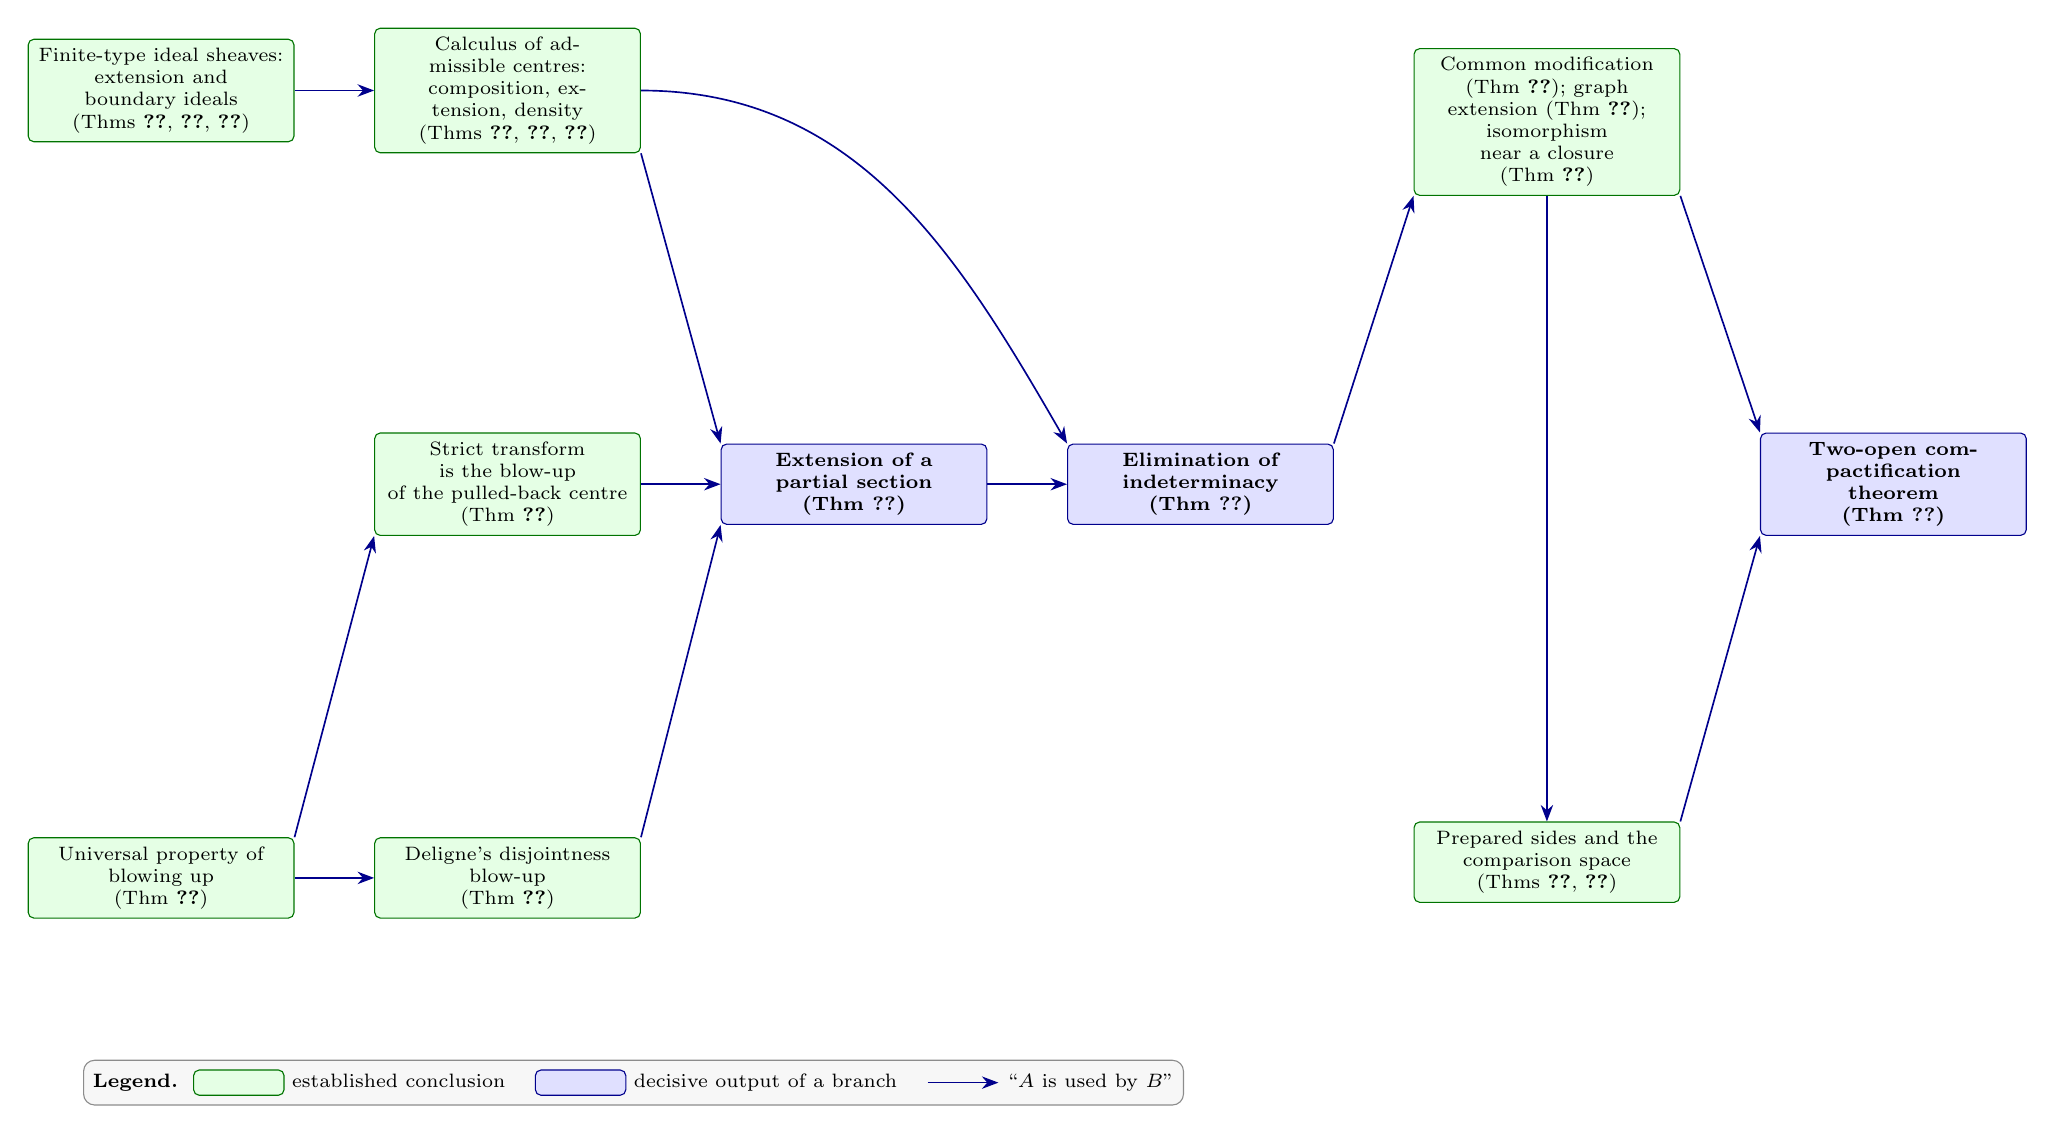
\begin{tikzpicture}

\node[est] (ft) at (0,5.0)
  {Finite-type ideal sheaves:\\ extension and boundary ideals\\
   (Thms~\ref{thm:01PF}, \ref{thm:finite-type-directed}, \ref{thm:01PH})};
\node[est] (up) at (0,-5.0)
  {Universal property of\\ blowing up\\ (Thm~\ref{thm:0806})};

\node[est] (adm) at (4.4,5.0)
  {Calculus of admissible centres:\\ composition, extension, density\\
   (Thms~\ref{thm:080B}, \ref{thm:080M}, \ref{thm:admissible-density})};
\node[est] (st) at (4.4,0)
  {Strict transform is the blow-up\\ of the pulled-back centre\\
   (Thm~\ref{thm:080E})};
\node[est] (dis) at (4.4,-5.0)
  {Deligne's disjointness\\ blow-up\\ (Thm~\ref{thm:disjointness})};

\node[key] (con) at (8.8,0)
  {Extension of a partial section\\ (Thm~\ref{thm:conrad24})};

\node[key] (eli) at (13.2,0)
  {Elimination of\\ indeterminacy\\ (Thm~\ref{thm:081S})};

\node[est] (mod) at (17.6,4.6)
  {Common modification\\ (Thm~\ref{thm:0F3X}); graph\\ extension (Thm~\ref{thm:0F3Z});\\
   isomorphism near a closure\\ (Thm~\ref{thm:0F3W})};
\node[est] (prep) at (17.6,-4.8)
  {Prepared sides and the\\ comparison space\\
   (Thms~\ref{thm:prepared-side}, \ref{thm:two-open-preparation})};

\node[key] (two) at (22.0,0)
  {Two-open compactification\\ theorem\\ (Thm~\ref{thm:two-open})};

\draw[dep] (ft) -- (adm);
\draw[dep] (up) -- (dis);
\draw[dep] (up.north east) -- (st.south west);
\draw[dep] (adm.south east) -- (con.north west);
\draw[dep] (st) -- (con);
\draw[dep] (dis.north east) -- (con.south west);
\draw[dep] (con) -- (eli);
\draw[dep] (adm.east) to[out=0,in=120] (eli.north west);
\draw[dep] (eli.north east) -- (mod.south west);
\draw[dep] (mod) -- (prep);
\draw[dep] (mod.south east) -- (two.north west);
\draw[dep] (prep.north east) -- (two.south west);

\node[draw=black!45, rounded corners, align=left, font=\scriptsize,
      fill=black!3] at (6.0,-7.6)
  {\textbf{Legend.}\ \ %
   \tikz[baseline=-0.6ex]\node[est,text width=1.05cm,minimum height=0.32cm,
     inner sep=1.4pt]{};\ established conclusion \quad
   \tikz[baseline=-0.6ex]\node[key,text width=1.05cm,minimum height=0.32cm,
     inner sep=1.4pt]{};\ decisive output of a branch \quad
   \tikz[baseline=-0.6ex]\draw[dep] (0,0)--(0.9,0);\ ``$A$ is used by $B$''};

\end{tikzpicture}
\end{adjustbox}
\end{center}
\end{landscape}

\begin{landscape}
\thispagestyle{empty}
\subsection*{Panel B. From the available ingredients to the target}

\begin{center}
\begin{adjustbox}{max width=\linewidth, max totalheight=0.90\textheight, center}
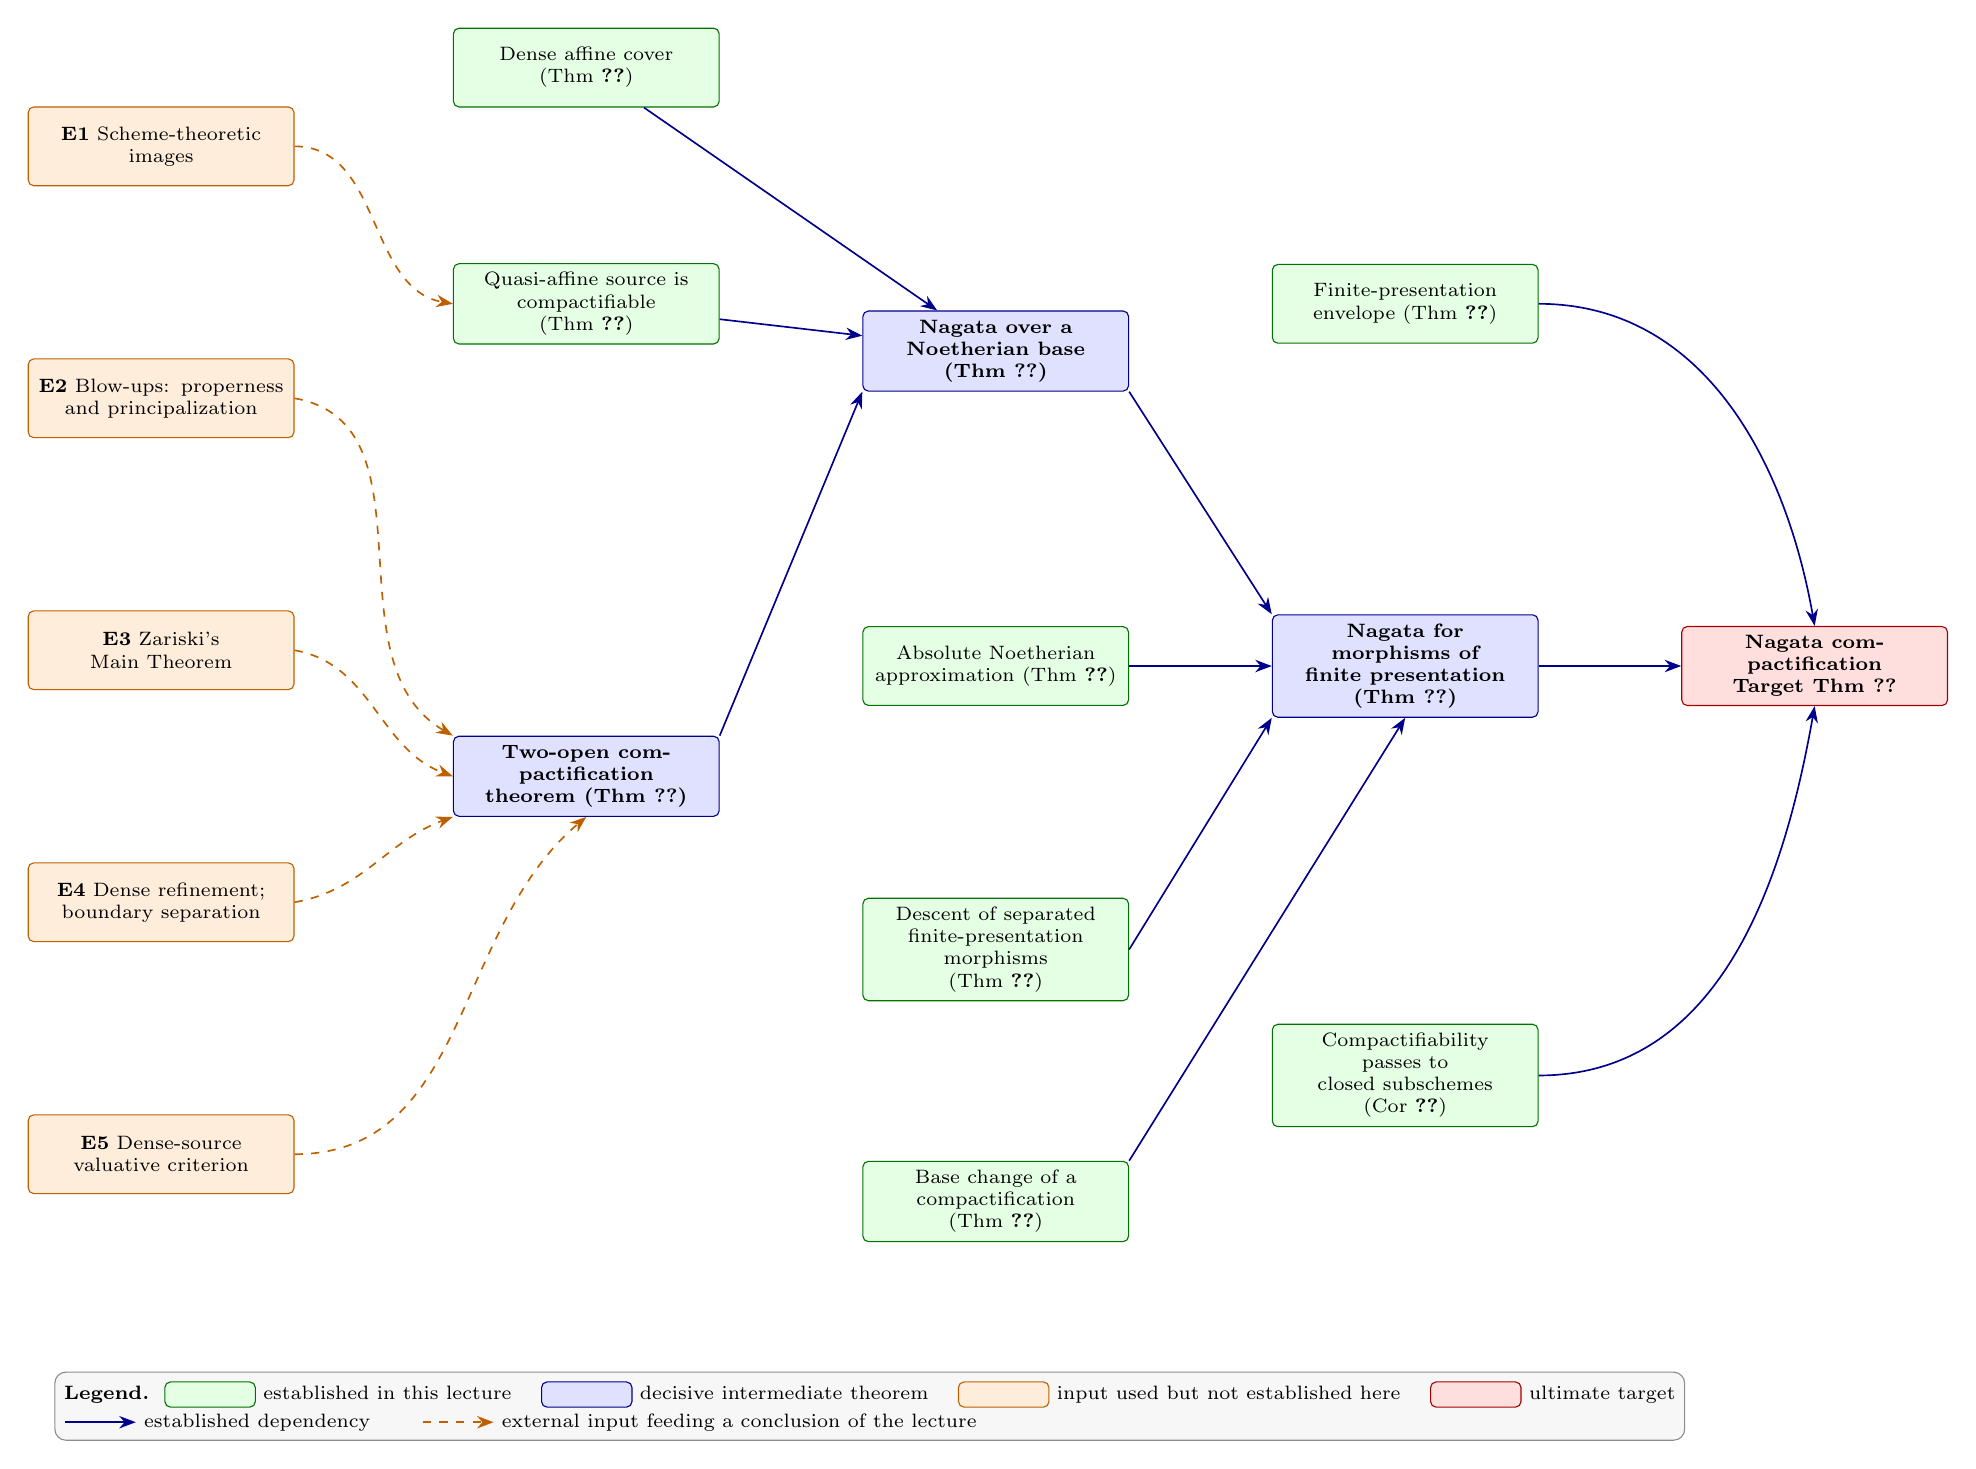
\begin{tikzpicture}

%% external inputs
\node[ext] (e1) at (0,5.6)
  {\textbf{E1} Scheme-theoretic\\ images};
\node[ext] (e2) at (0,2.4)
  {\textbf{E2} Blow-ups: properness\\ and principalization};
\node[ext] (e3) at (0,-0.8)
  {\textbf{E3} Zariski's\\ Main Theorem};
\node[ext] (e4) at (0,-4.0)
  {\textbf{E4} Dense refinement;\\ boundary separation};
\node[ext] (e5) at (0,-7.2)
  {\textbf{E5} Dense-source\\ valuative criterion};

%% available ingredients
\node[key] (two) at (5.4,-2.4)
  {Two-open compactification\\ theorem (Thm~\ref{thm:two-open})};
\node[est] (aff) at (5.4,3.6)
  {Quasi-affine source is\\ compactifiable\\ (Thm~\ref{thm:quasi-affine-compactifiable})};
\node[est] (cov) at (5.4,6.6)
  {Dense affine cover\\ (Thm~\ref{thm:dense-affine-cover})};

\node[key] (noe) at (10.6,3.0)
  {Nagata over a\\ Noetherian base\\ (Thm~\ref{thm:noetherian})};
\node[est] (app) at (10.6,-1.0)
  {Absolute Noetherian\\ approximation (Thm~\ref{thm:01ZA})};
\node[est] (desc) at (10.6,-4.6)
  {Descent of separated\\ finite-presentation morphisms\\ (Thm~\ref{thm:01ZQ})};
\node[est] (bc) at (10.6,-7.8)
  {Base change of a\\ compactification\\ (Thm~\ref{thm:base-change})};

\node[key] (fp) at (15.8,-1.0)
  {Nagata for morphisms of\\ finite presentation\\ (Thm~\ref{thm:fp-nagata})};
\node[est] (env) at (15.8,3.6)
  {Finite-presentation\\ envelope (Thm~\ref{thm:01ZJ})};
\node[est] (cls) at (15.8,-6.2)
  {Compactifiability passes to\\ closed subschemes\\ (Cor~\ref{cor:closed-subscheme})};

\node[goal] (goal) at (21.0,-1.0)
  {\textbf{Nagata compactification}\\ Target Thm~\ref{thm:nagata}};

\draw[dep] (cov) -- (noe);
\draw[dep] (aff) -- (noe);
\draw[dep] (two.north east) -- (noe.south west);
\draw[dep] (noe.south east) -- (fp.north west);
\draw[dep] (app) -- (fp);
\draw[dep] (desc.east) -- (fp.south west);
\draw[dep] (bc.north east) -- (fp.south);
\draw[dep] (fp) -- (goal);
\draw[dep] (env.east) to[out=0,in=100] (goal.north);
\draw[dep] (cls.east) to[out=0,in=-100] (goal.south);

\draw[extdep] (e1.east) to[out=0,in=170] (aff.west);
\draw[extdep] (e2.east) to[out=-10,in=150] (two.north west);
\draw[extdep] (e3.east) to[out=-10,in=160] (two.west);
\draw[extdep] (e4.east) to[out=10,in=-160] (two.south west);
\draw[extdep] (e5.east) to[out=0,in=-140] (two.south);

\node[draw=black!45, rounded corners, align=left, font=\scriptsize,
      fill=black!3] at (9.0,-10.4)
  {\textbf{Legend.}\ \ %
   \tikz[baseline=-0.6ex]\node[est,text width=1.05cm,minimum height=0.32cm,
     inner sep=1.4pt]{};\ established in this lecture \quad
   \tikz[baseline=-0.6ex]\node[key,text width=1.05cm,minimum height=0.32cm,
     inner sep=1.4pt]{};\ decisive intermediate theorem \quad
   \tikz[baseline=-0.6ex]\node[ext,text width=1.05cm,minimum height=0.32cm,
     inner sep=1.4pt]{};\ input used but not established here \quad
   \tikz[baseline=-0.6ex]\node[goal,text width=1.05cm,minimum height=0.32cm,
     inner sep=1.4pt]{};\ ultimate target\\[2pt]
   \tikz[baseline=-0.6ex]\draw[dep] (0,0)--(0.9,0);\ established dependency
   \qquad
   \tikz[baseline=-0.6ex]\draw[extdep] (0,0)--(0.9,0);\ external input feeding a
   conclusion of the lecture};

\end{tikzpicture}
\end{adjustbox}
\end{center}
\end{landscape}

\end{document}
